%#! platex UserGuideJa
\chapter{チュートリアル}
\label{chap:2}
この章ではOpenFOAMを動かす基本的な手順をユーザに説明することを主な目標として,
OpenFOAMのいくつかのテストケースで,設定,
シミュレーション,および後処理のプロセスを詳しく記述します.
\OFpath{\$FOAM\_TUTORIALS}のディレクトリには
OpenFOAMが提供するすべてのソルバと
多くのユーティリティを使い方を示す数多くのケースがあります.
チュートリアルを始める前にユーザは最初にOpenFOAMが正しく
インストールされていることを確かめなければなりません.

チュートリアルのケースは\OFtool{blockMesh}の前処理ツールを使用して記述し,
OpenFOAMのソルバで動かし,\OFtool{paraFoam}を使用して後処理を行います.
OpenFOAMのサポートするサードパーティの後処理ツールでアクセスする
ユーザには次の選択肢があります.
\OFtool{paraFoam}を使用しチュートリアルを進めるか,
または後処理が必要な際に
\autoref{chap:6}で述べるサードパーティ製品の使い方を参照するかです.

すべてのチュートリアルのコピーは
OpenFOAMをインストールしたチュートリアルのディレクトリから利用できます.
チュートリアルは,流れのタイプによるディレクトリと
ソルバのサブディレクトリにまとめられています.
例えば
\index{icoFoam@\OFtool{icoFoam}!ソルバ}%
\index{ソルバ!icoFoam@\OFtool{icoFoam}}%
\OFtool{icoFoam}のケースはすべて
\OFpath{incompressible/icoFoam}サブディレクトリの中に置かれています.
ここでincompressibleが流れのタイプを表しています.
ユーザがさまざまな例題を実施するときには,
\index{tutorials@\OFpath{tutorials}!ディレクトリ}%
\index{ディレクトリ!tutorials@\OFpath{tutorials}}%
\OFpath{tutorials}ディレクトリをローカルの実行ディレクトリに
コピーすることをお勧めします.
そのためには,次のようにタイプすることで容易にコピーすることができます.
\begin{OFverbatim}[terminal]
mkdir -p $FOAM_RUN
cp -r $FOAM_TUTORIALS $FOAM_RUN
\end{OFverbatim}%$



\section{天井駆動のキャビティ流れ}
\label{sec:2.1}
\index{てんじょうくどうのキャビティながれ@天井駆動のキャビティ流れ}%
\index{チュートリアル!てんじょうくどうのキャビティながれ@天井駆動のキャビティ流れ}%
\index{キャビティながれ@キャビティ流れ}%
このチュートリアルは2次元正方形領域の等温非圧縮性流れに関して,
プリプロセス,計算,ポストプロセスする方法を解説します.
\autoref{fig:2.1}に
正方形のすべての境界が壁面境界であるジオメトリを示します.
上の壁面境界は$x$軸方向に$1\unit{m/s}$の速度ではたらき,
他の三つの壁面境界は静止しています.
チュートリアルにおいてはこれを解くにあたって,まず
\index{ながれ@流れ!そうりゅう@層流}%
層流を仮定し,
層流等温非圧縮性流れのための\OFtool{icoFoam}ソルバを使用し
均一メッシュ上で解きます.
チュートリアルでは,
メッシュの解像度の増加や壁方向への勾配の影響を調べます.
これにより流れの
\index{レイノルズすう@レイノルズ数}%
レイノルズ数を増加させ,
\index{pisoFoam@\OFtool{pisoFoam}!ソルバ}%
\index{ソルバ!pisoFoam@\OFtool{pisoFoam}}%
\OFtool{pisoFoam}ソルバを
\index{ながれ@流れ!らんりゅう@乱流}%
乱流,等温,非圧縮性流れに使用します.


\begin{figure}[ht]
 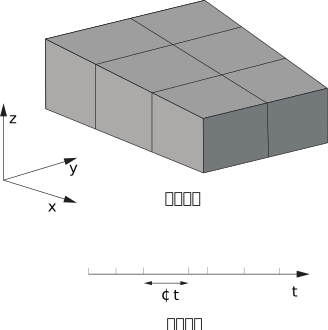
\includegraphics{fig-2-1}
 \caption{天井駆動キャビティのジオメトリ}
 \label{fig:2.1}
\end{figure}


\subsection{前処理}
\label{ssec:2.1.1}
ケースはOpenFOAMでケースファイルを編集することで設定します.
ケースファイルは\OFthirdparty{emacs}や\OFthirdparty{vi},
\OFthirdparty{gedit},\OFthirdparty{kate},\OFthirdparty{nedit}などの
テキストエディタで作成・編集します.
それは,入出力が初心者でもわかりやすいキーワードをもつ
ディクショナリ形式が使われているからです.

解析ケースはメッシュ,物理量,物性,制御パラメータなどの要素を
含んでいますが\autoref{sec:4.1}において示すように,
多くのCFDソフトが一つのファイルにこれらのデータを格納するのに対し,
OpenFOAMは一連のファイルセットとして解析ケースディレクトリに格納します.
解析ケースのディレクトリには,
(最初のチュートリアルの例題が単純にcavityであるように)
わかりやすい名前を与えます.
解析ケースを編集・実行する前の準備として,
まず解析対象のディレクトリに移動します.
\begin{OFverbatim}[terminal]
cd $FOAM_RUN/tutorials/incompressible/icoFoam/cavity
\end{OFverbatim}%$

\subsubsection{メッシュ生成}
\label{sssec:2.1.1.1}
\index{ざひょうじく@座標軸!みぎてけいちょっこうデカルト@右手系直交デカルト}%
OpenFOAMは常に3次元デカルト
\index{ざひょうけい@座標系}%
座標系で動くため,
全てのジオメトリを3次元で生成します.
OpenFOAMはデフォルトの設定において問題を3次元として解きますが,
2次元を解く場合は,解決が必要でない(第3)次元方向に垂直な境界に
\textgt{特別な}
\index{empty@\OFboundary{empty}!きょうかいじょうけん@境界条件}%
\index{きょうかいじょうけん@境界条件!empty@\OFboundary{empty}}%
\OFboundary{empty}という境界条件を指定します.

$x$--$y$平面上の一辺の長さの正方形からなるキャビティの領域に,
まず$20 \times 20$セルの均一なメッシュを設定します.
このブロック構造を\autoref{fig:2.2}に示します.


\begin{figure}[ht]
 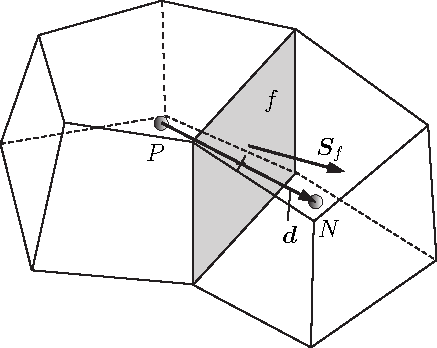
\includegraphics{fig-2-2}
 \caption{キャビティのメッシュのブロック構造}
 \label{fig:2.2}
\end{figure}


OpenFOAMで提供されるメッシュ・ジェネレータ\OFtool{blockMesh}は
\OFpath{constant/polyMesh}ディレクトリにある入力ディクショナリ
\index{blockMeshDict@\OFdictionary{blockMeshDict}!ディクショナリ}%
\index{ディクショナリ!blockMeshDict@\OFdictionary{blockMeshDict}}%
\OFdictionary{blockMeshDict}で指定された
記述からメッシュを生成します.
このケースの\OFdictionary{blockMeshDict}は,以下のとおりです.
\begin{OFverbatim}[file, linenum]
/*--------------------------------*- C++ -*----------------------------------*\
| =========                 |                                                 |
| \\      /  F ield         | OpenFOAM: The Open Source CFD Toolbox           |
|  \\    /   O peration     | Version:  2.0.0                                 |
|   \\  /    A nd           | Web:      www.OpenFOAM.com                      |
|    \\/     M anipulation  |                                                 |
\*---------------------------------------------------------------------------*/
FoamFile
{
    version     2.0;
    format      ascii;
    class       dictionary;
    object      blockMeshDict;
}
// * * * * * * * * * * * * * * * * * * * * * * * * * * * * * * * * * * * * * //

convertToMeters 0.1;

vertices        
(
    (0 0 0)
    (1 0 0)
    (1 1 0)
    (0 1 0)
    (0 0 0.1)
    (1 0 0.1)
    (1 1 0.1)
    (0 1 0.1)
);

blocks          
(
    hex (0 1 2 3 4 5 6 7) (20 20 1) simpleGrading (1 1 1)
);

edges           
(
);

boundary
(

    movingWall 
    {
        type wall;
        faces
        (
            (3 7 6 2)
        );
    }
    fixedWalls 
    {
        type wall;
        faces
        (
            (0 4 7 3)
            (2 6 5 1)
            (1 5 4 0)
        );
    }
    frontAndBack 
    {
        type empty;
        faces
        (
            (0 3 2 1)
            (4 5 6 7)
        );
    }
);

mergePatchPairs 
(
);

// ************************************************************************* //
\end{OFverbatim}
ファイルの最初はバナー(1--7行)形式のヘッダ情報で,
ファイル情報は,波括弧 (\verb|{|\ldots\verb|}|) で囲まれる
\OFsubdictionary{FoamFile}サブディクショナリの中で記述されます.

今後は,簡便化とスペースの都合上,
バナーと\OFsubdictionary{FoamFile}サブディクショナリを含む
ファイルヘッダはケースファイルの引用の際に省きます.

まずファイルは初めにブロックの頂点の座標
\index{vertices@\OFkeyword{vertices}!キーワード}%
\index{キーワード!vertices@\OFkeyword{vertices}}%
\OFkeyword{vertices}を指定します.
それに続き,頂点名とセル番号から
\index{blocks@\OFkeyword{blocks}!キーワード}%
\index{キーワード!blocks@\OFkeyword{blocks}}%
\OFkeyword{blocks}(ここでは一つのみ)を定義します.
そして最後に境界パッチを定義します.
\OFdictionary{blockMeshDict}ファイルの記述の詳細を理解するには
\autoref{sec:5.3}を参照してください.

メッシュは\OFdictionary{blockMeshDict}ファイル上で
\OFtool{blockMesh}を実行すると生成されます.
ケースディレクトリ内から以下をターミナルに入力するだけです.
\begin{OFverbatim}[terminal]
blockMesh
\end{OFverbatim}
\OFtool{blockMesh}の実行状況はターミナルウィンドウに表示されます.
\index{blockMeshDict@\OFdictionary{blockMeshDict}!ディクショナリ}%
\index{ディクショナリ!blockMeshDict@\OFdictionary{blockMeshDict}}%
\OFdictionary{blockMeshDict}ファイルに誤りがあった場合,
エラーメッセージが表示され,
ファイルのどの行に問題があるかを教えてくれます.
今この段階でエラーメッセージが出ることはないでしょう.

\subsubsection{境界条件と初期条件}
\label{sssec:2.1.1.2}
メッシュの生成が完了すると,物理的条件の初期状態を確認することができます.
このケースは開始時刻がに設定されているので解析領域の初期状態のデータは
\OFpath{cavity}ディレクトリの\OFpath{0}という
サブディレクトリに格納されています.
\OFpath{0}には\OFpath{p}と\OFpath{U}の二つのファイルがあり,
圧力 ($p$) と速度 ($U$) の初期値と境界条件を設定する必要があります.
\OFpath{p}のファイルを例に説明します.
\begin{OFverbatim}[file, linenum=17]
dimensions      [0 2 -2 0 0 0 0];

internalField   uniform 0;

boundaryField
{
    movingWall
    {
        type            zeroGradient;
    }

    fixedWalls
    {
        type            zeroGradient;
    }

    frontAndBack
    {
        type            empty;
    }
}

// ************************************************************************* //
\end{OFverbatim}
物理的条件のデータファイルには三つの主要な項目があります.
\begin{description}
 \item[dimensions]
\index{dimensions@\OFkeyword{dimensions}!キーワード}%
\index{キーワード!dimensions@\OFkeyword{dimensions}}%
            物理量の次元を定義.ここでは動圧,
            つまり$\unit*{m^{2}s^{-2}}$(\autoref{ssec:4.2.6}に詳述).
 \item[internalField]
\index{internalField@\OFkeyword{internalField}!キーワード}%
\index{キーワード!internalField@\OFkeyword{internalField}}%
            内部の物理量は単一の値で記述すれば一様となり,
            一様でない場合はすべての値を指定する必要があります
            (\autoref{ssec:4.2.8}に詳述).
 \item[boundaryField]
\index{boundaryField@\OFkeyword{boundaryField}!キーワード}%
\index{キーワード!boundaryField@\OFkeyword{boundaryField}}%
            境界面の物理量は境界条件と境界パッチに与えるデータを
            記述します(\autoref{ssec:4.2.8}に詳述).
\end{description}
このキャビティ流れの解析ケースでは境界は壁面のみですが,
二つのパッチが使用されています.
(1) キャビティの固定された側面と底面用の\OFpatch{fixedwall}と,
(2) キャビティの駆動天井面用の\OFpatch{movingwall}です.
どちらも$p$が\OFkeyword{zeroGradient}ですが,
これは圧力の境界に垂直な方向の勾配が$0$であるということです.
\OFpatch{frontAndBack}は2次元の問題の場合の表裏の平面を示していて,
本ケースでは当然\OFkeyword{empty}となっています.

このケースでは,もっともよく目にするものでありますが,
物理量の初期条件が\OFkeyword{uniform}(一様)になっています.
ここでは圧力は動圧のみの非圧縮ケースであるため,
絶対値は解析と関係ないので便宜上\texttt{uniform 0}としています.

\OFpath{0/U}の速度のファイルにおいても同様です.
\OFkeyword{dimensions}は速度であり,
内部の初期条件はベクトル量で3成分とも$0$を意味する
\texttt{uniform (0 0 0)}になっています(\autoref{ssec:4.2.5}に詳述).

速度の境界条件は\OFpatch{frontAndBack}パッチと同じ条件です.
\OFpatch{fixedWall}に関してはすべりなしのため
\index{value@\OFkeyword{value}!キーワード}%
\index{キーワード!value@\OFkeyword{value}}%
\OFkeyword{value}は\texttt{uniform (0 0 0)}となります.
上面は$1\unit{m/s}$で移動するので\texttt{uniform (1 0 0)}で固定値を設定します.

\subsubsection{物性値}
\label{sssec:2.1.1.3}
ケースの物理量は,名前に\OFpath{...Properties}という語尾を与えられて
ディクショナリに保存され,\OFpath{Dictionaries}ディレクトリツリーに置かれます.
\index{icoFoam@\OFtool{icoFoam}!ソルバ}%
\index{ソルバ!icoFoam@\OFtool{icoFoam}}%
\OFtool{icoFoam}ケースでは,
\index{transportProperties@\OFdictionary{transportProperties}!ディクショナリ}%
\index{ディクショナリ!transportProperties@\OFdictionary{transportProperties}}%
\OFdictionary{transportProperties}ディクショナリに保存される
動粘性係数を指定するだけです.
\OFdictionary{transportProperties}ディクショナリを開いてエントリを見たり,
編集することができますので,
\index{ねんせいけいすう@粘性係数!どう@動\jdash}%
動粘性係数が正しくセットされることを確かめてください.
動粘性係数は,\OFkeyword{nu} (方程式で見られる
ギリシア語シンボル$\nu$の音声ラベル)
というキーワードになります.
まず最初に,このケースはレイノルズ数を$10$で計算します.
\index{レイノルズすう@レイノルズ数}%
レイノルズ数は次のように定義されます.
\begin{align}
 \label{eq:2.1}
 \nRe = \frac{d|\bm{U}|}{\nu}
\end{align}
$d$と$\bm{U}$はそれぞれ特性長さと速度を表し,
$\nu$は動粘性係数を表します.
ここで,$d = 0.1\unit{m}$,$|\bm{U}| = 1\unit{m\,s^{-1}}$,
$\nRe = 10$とすると,$\nu = 0.01\unit{m^{2}s^{-1}}$となります.
動粘性係数の適切な設定は以下のようになります.
\begin{OFverbatim}[file, linenum=17]

nu              nu [0 2 -1 0 0 0 0] 0.01;


// ************************************************************************* //
\end{OFverbatim}

\subsubsection{制御}
\label{sssec:2.1.1.4}
計算時間の制御,解のデータの読み書きに関する入力データは,
\index{controlDict@\OFdictionary{controlDict}!ディクショナリ}%
\index{ディクショナリ!controlDict@\OFdictionary{controlDict}}%
\OFdictionary{controlDict}ディクショナリから読み取られます.
これは\OFpath{system}ディレクトリにありますので,
ケースを制御するファイルとして参照してください.

まず最初にスタート・停止時刻と時間ステップを設定しなければなりません.
OpenFOAMは,柔軟性の高い時間制御を提供しますが,
詳しくは\autoref{sec:4.3}で述べます.このチュートリアルでは,
時刻$t = 0$から実行を始めたいと思います.
つまり,OpenFOAMは\OFpath{0}というディレクトリから
場のデータを読む必要があることになります
(ケースファイル構造の詳しい情報に関しては\autoref{sec:4.1}を見てください).
したがって,
\index{startFrom@\OFkeyword{startFrom}!キーワード}%
\index{キーワード!startFrom@\OFkeyword{startFrom}}%
\OFkeyword{startFrom}キーワードを
\index{startTime@\OFkeyword{startTime}!キーワードエントリ}%
\index{キーワードエントリ!startTime@\OFkeyword{startTime}}%
\OFkeyword{startTime}に設定して,
次に
\index{startTime@\OFkeyword{startTime}!キーワード}%
\index{キーワード!startTime@\OFkeyword{startTime}}%
\OFkeyword{startTime}キーワードを0に指定します.

終了時刻には,流れがキャビティ周りを循環している定常解に達することを
目標にするわけですが,概して,流体は層流で定常状態に到達するために
領域を10回通り抜けなければなりません.
このケースでは,入口も出口もないので,流れが解析領域を通り抜けません.
代わりに,ふたがキャビティを10回移動する時刻 (すなわち$1\unit{s}$) を
終了時刻としてセットしてもいいでしょう.
実際は,後の知見により,$0.5\unit{s}$で十分であるとわかるので,
この値を採用しましょう.
この終了時刻を指定するために,\OFkeyword{stopAt}キーワードとして
\OFkeyword{endTime}を指定して,
\index{endTime@\OFkeyword{endTime}!キーワード}%
\index{キーワード!endTime@\OFkeyword{endTime}}%
\OFkeyword{endTime}キーワードを0.5に設定しなければなりません.

次に,時間ステップを設定する必要がありますが,
これはキーワード\OFkeyword{deltaT}によって表されます.
\OFtool{icoFoam}を動かすとき,時間の精度と安定性を達成するために,
$1$未満のクーラン数が必要です.
\index{クーランすう@クーラン数}%
クーラン数は以下のように定義されます.
\begin{align}
 \label{eq:2.2}
  \nCo = \frac{\Delta t|\bm{U}|}{\Delta x}
\end{align}
$\Delta t$は時間ステップ,$|\bm{U}|$はセルを通る流速の大きさ,
そして$\Delta x$は流速方向のセルサイズです.
流速が領域内で変化しても必ず$\nCo < 1$を成り立たせる必要があります.
だから,最も悪い場合(つまり,大きな流速と小さなセルサイズの
組合わせによる最大の$\nCo$)を元に$\Delta t$を決定します.
ここでは,セルサイズは解析領域中全域で固定されているので,
最大$\nCo$はふた付近に生じ,$1\unit{m\,s^{-1}}$に近い流速になるでしょう.
\begin{align}
 \label{eq:2.3}
  \Delta x = \frac{d}{n} = \frac{0.1}{20} = 0.005\unit{m}
\end{align}
したがって,領域中で$1$以下のクーラン数を達成するために,
\index{じかんステップ@時間ステップ}%
時間ステップ\OFkeyword{deltaT}を次のように設定しなくてはいけません.
\begin{align}
 \label{eq:2.4}
  \Delta t = \frac{\nCo\Delta x}{|\bm{U}|}
  = \frac{1 \times 0.005}{1} = 0.005\unit{s}
\end{align}
シミュレーションが進行するとき,
後処理パッケージで後から見ることができるように,
ある一定の時間間隔での結果の書き出しをもとめるため,
\index{writeControl@\OFkeyword{writeControl}!キーワード}%
\index{キーワード!writeControl@\OFkeyword{writeControl}}%
\OFkeyword{writeControl}キーワードは結果が書かれる時刻を決めるための
いくつかのオプションを提示します.
\index{timeStep@\OFkeyword{timeStep}!キーワードエントリ}%
\index{キーワードエントリ!timeStep@\OFkeyword{timeStep}}%
\OFkeyword{timeStep}オプションは,
結果が$n$回の時間ステップごとに結果を書き出すということを意味し,
そのときの値は
\index{writeInterval@\OFkeyword{writeInterval}!キーワード}%
\index{キーワード!writeInterval@\OFkeyword{writeInterval}}%
\OFkeyword{writeInterval}キーワードで指定されます.
$0.1, 0.2, \ldots, 0.5\unit{s}$で結果を書きたいとしましょう.
したがって,$0.005\unit{s}$の時間ステップなので,
時間ステップ$20$回ごとに結果を出力する必要があります.
よって\OFkeyword{writeInterval}に20を設定します.

OpenFOAMは\autoref{sec:4.1}で議論するデータセットを
書き込むごとに例えば$0.1\unit{s}$という現在時刻にちなんで名付けられた
新しいディレクトリを作成します.
\index{icoFoam@\OFtool{icoFoam}!ソルバ}%
\index{ソルバ!icoFoam@\OFtool{icoFoam}}%
\OFtool{icoFoam}ソルバでは,
\index{U@\OFkeyword{U}!フィールド}%
\index{フィールド!U@\OFkeyword{U}}%
\OFkeyword{U}や
\index{p@\OFkeyword{p}!フィールド}%
\index{フィールド!p@\OFkeyword{p}}%
\OFkeyword{p}の各項目ごとに結果を時刻ディレクトリに書き込みます.
このケースでは,\OFdictionary{controlDict}の記述内容は以下のとおりです.
\begin{OFverbatim}[file, linenum=17]

application     icoFoam;

startFrom       startTime;

startTime       0;

stopAt          endTime;

endTime         0.5;

deltaT          0.005;

writeControl    timeStep;

writeInterval   20;

purgeWrite      0;

writeFormat     ascii;

writePrecision  6;

writeCompression off;

timeFormat      general;

timePrecision   6;

runTimeModifiable true;


// ************************************************************************* //
\end{OFverbatim}

\subsubsection{離散化と線形ソルバの設定}
\label{sssec:2.1.1.5}
ユーザは\OFdictionary{fvSchemes}ディクショナリ (\OFpath{system}ディレクトリ) 内で
有限体積離散化法を選択するかどうか指定します.
線形方程式ソルバと許容値および他のアルゴリズムコントロールの指定は
\OFdictionary{fvSolution}ディクショナリ内に作られています.
ユーザは自由にこれらのディクショナリを見ることができますが,
\OFdictionary{fvSolution}ディクショナリの
\index{PISO@\OFsubdictionary{PISO}!ディクショナリ}%
\index{ディクショナリ!PISO@\OFsubdictionary{PISO}}%
\OFsubdictionary{PISO}サブディクショナリの
\index{pRefCell@\OFkeyword{pRefCell}!キーワード}%
\index{キーワード!pRefCell@\OFkeyword{pRefCell}}%
\OFkeyword{pRefCell}と
\index{pRefValue@\OFkeyword{pRefValue}!キーワード}%
\index{キーワード!pRefValue@\OFkeyword{pRefValue}}%
\OFkeyword{pRefValue}を除いて,
現在のところ,それらすべての項について議論する必要はありません.
キャビティのような閉じた非圧縮系では,圧力は相対的であり,
重要なのは(絶対値ではなく)圧力範囲です.
このような場合では,ソルバはセル\OFkeyword{pRefCell}に\OFkeyword{pRefValue}による
参照レベルをセットします.この例では,両方が0に設定されます.
しかし,これらの値のどちらかを変えると絶対圧力
(速度と相対圧力ではなく)が変化します.


\subsection{メッシュの確認}
\label{ssec:2.1.2}
解析を実行する前に正しくメッシュができているか確認しましょう.
メッシュはOpenFoamが提供する後処理ソフトの
\index{paraFoam@\OFtool{paraFoam}}%
\OFtool{paraFoam}で確認します.
\OFtool{paraFoam}は解析ケースのディレクトリ上でターミナルから起動します.
\begin{OFverbatim}[terminal]
paraFoam
\end{OFverbatim}
あるいは,オプションに\texttt{-case}をつけることで
他のディレクトリからでも起動することができます.
\begin{OFverbatim}[terminal]
paraFoam -case $FOAM_RUN/tutorials/incompressible/icoFoam/cavity
\end{OFverbatim}%$

\autoref{fig:6.1}に示すように\OFthirdparty{ParaView}のウィンドウが開きます.
\index{Pipeline Browser@\PVwindow{Pipeline Browser}!ウィンドウ}%
\index{ウィンドウ!Pipeline Browser@\PVwindow{Pipeline Browser}}%
\PVwindow{Pipeline Browser}を見ると,\OFthirdparty{ParaView}が\PVkeyword{cavity.OpenFOAM},
つまりキャビティケースのモデュールを開いていることが確認できます.
\emph{\PVbutton{Apply}ボタンをクリックする前に}%
\index{Mesh Parts@\PVpanel{Mesh Parts}!ウィンドウパネル}%
\index{ウィンドウパネル!Mesh Parts@\PVpanel{Mesh Parts}}%
\PVpanel{Mesh Parts}パネルから
表示する要素を選択する必要があります.
解析ケースが単純なので\PVpanel{Mesh Parts}パネルのチェックボックスで
全てのデータを選択することが簡単です.
パネル内の全要素を自動的にチェックすることができます.
\OFthirdparty{ParaView}でジオメトリを読込むためには\PVbutton{Apply}ボタンをクリックします.

最初から適用されている一般的な設定については
\autoref{sssec:6.1.5.1}を参照してください.

\index{Display@\PVpanel{Display}!ウィンドウパネル}%
\index{ウィンドウパネル!Display@\PVpanel{Display}}%
\PVpanel{Display}タブを開き選択したモジュールの表示形式を調整します.
\autoref{fig:2.3}に示すように,
(1) \PVkeyword{Color by}を\PVkeyword{Solid Color}に設定し,
(2) \PVbutton{Set Solid Color}をクリックし適当な色(背景が白の場合は黒など)を選択,
(3)\ 
\index{Style@\PVpanel{Style}!ウィンドウパネル}%
\index{ウィンドウパネル!Style@\PVpanel{Style}}%
\PVpanel{Style}パネルでは\PVkeyword{Representation}メニューから
\PVkeyword{Wireframe}を選択します.
背景色はトップメニューパネルで\PVkeyword{Edit}から
\index{View Settings...@\PVkeyword{View Settings...}!メニューエントリ}%
\index{メニューエントリ!View Settings...@\PVkeyword{View Settings...}}%
\PVkeyword{View Settings...}を選択して設定します.


\begin{figure}[ht]
 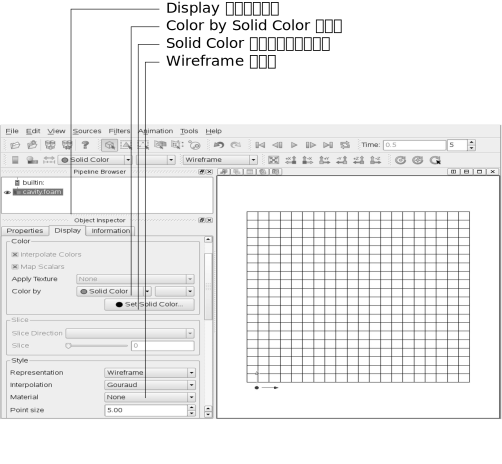
\includegraphics{fig-2-3}
 \caption{paraFoamでのメッシュの表示}
 \label{fig:2.3}
\end{figure}


\OFthirdparty{ParaView}を使うのがはじめてならば,
\autoref{ssec:6.1.5}で述べるように視点操作を試してみることをお勧めします.
特に本ケースは2次元なので\PVkeyword{Edit}メニューの
\index{View Settings@\PVkeyword{View Settings}!メニューエントリ}%
\index{メニューエントリ!View Settings@\PVkeyword{View Settings}}%
\PVkeyword{View Settings}のGeneralパネルで
\index{Use Parallel Projection@\PVbutton{Use Parallel Projection}!ボタン}%
\index{ボタン!Use Parallel Projection@\PVbutton{Use Parallel Projection}}%
\PVbutton{Use Parallel Projection}を
選択するのがよいでしょう.
軸の方向は,
\index{Annotation@\PVpanel{Annotation}!ウィンドウパネル}%
\index{ウィンドウパネル!Annotation@\PVpanel{Annotation}}%
\PVpanel{Annotation}ウィンドウの
\index{Orientation Axes@\PVbutton{Orientation Axes}!ボタン}%
\index{ボタン!Orientation Axes@\PVbutton{Orientation Axes}}%
\PVbutton{Orientation Axes}をオン・オフするか,
マウスのドラッグ\&ドロップによって操作することができます.


\subsection{アプリケーションの実行}
\label{ssec:2.1.3}
あらゆるUNIX/Linuxの実行ファイルと同様に,
OpenFOAMアプリケーションは二つの方法で実行することができます.
一つ目は
\index{フォアグラウンド!プロセス}%
\index{プロセス!フォアグラウンド}%
フォアグラウンドのプロセスで,
コマンドプロンプトを与えるのにシェルが命令終了まで待つものです.
二つ目は
\index{バックグラウンド!プロセス}%
\index{プロセス!バックグラウンド}%
バックグラウンドプロセスで,
シェルがさらなる命令を受け入れるのに命令完了の必要がないものです.

ここでは,フォアグランドで
\index{icoFoam@\OFtool{icoFoam}!ソルバ}%
\index{ソルバ!icoFoam@\OFtool{icoFoam}}%
\OFtool{icoFoam}を動かしましょう.
\OFtool{icoFoam}ソルバはケースディレクトリ内に入って,
コマンドプロンプト上で
\begin{OFverbatim}[terminal]
icoFoam
\end{OFverbatim}
と入力することで実行できますが,

あるいはオプションに\texttt{-case}をつけることで
他のディレクトリからでも起動することができます.
\begin{OFverbatim}[terminal]
icoFoam -case $FOAM_RUN/tutorials/incompressible/icoFoam/cavity
\end{OFverbatim}%$
ジョブの進捗は,ターミナルウィンドウに表示されます.
現在の時刻,最大クーラン数,全てのフィールドの初期値と最終的結果を表示します.


\subsection{後処理}
\label{ssec:2.1.4}
結果が時刻ディレクトリに書かれるとすぐに,
\OFtool{paraFoam}を使って見ることができます.
\OFtool{para\-Foam}ウィンドウに戻って,
\texttt{cavity.OpenFOAM}ケースモジュールの
\index{Properties@\PVpanel{Properties}!ウィンドウパネル}%
\index{ウィンドウパネル!Properties@\PVpanel{Properties}}%
\PVpanel{Properties}パネルを選んでください.
ケースモジュールのパネルが存在していないようならば,
\texttt{cavity.OpenFOAM}が青くハイライトされているか,
それと並んだ目のボタンは表示が有効であることを示しているか,
を確認してください.

見たいデータを表示する\OFtool{paraFoam}を準備するには,
最初に必須の実行時間として$0.5\unit{s}$分のデータを読込まなければなりません.
ケースが実行中で一方\OFthirdparty{ParaView}を開いている場合,
時間ディレクトリの出力データは\OFthirdparty{ParaView}に自動的にロードはされません.
データをロードするためには,\PVwindow{Properties}ウィンドウで
\index{Refresh Times@\PVbutton{Refresh Times}!ボタン}%
\index{ボタン!Refresh Times@\PVbutton{Refresh Times}}%
\PVbutton{Refresh Times}をクリックします.
これで各時刻のデータが\OFthirdparty{ParaView}にロードされます.

\subsubsection{等値面とコンタプロット}
\label{sssec:2.1.4.1}
圧力を見るには
\index{Display@\PVpanel{Display}!ウィンドウパネル}%
\index{ウィンドウパネル!Display@\PVpanel{Display}}%
\PVpanel{Display}パネルを開き,
選択したモジュールの表示形式を調整します.
圧力分布を見るには\autoref{fig:2.4}に示すように
\PVpanel{Style}パネルのRepresentationメニューをsurfaceにして
ColorPanelのSet Color byを 
\includegraphics{icon-point-p},
そして
\index{Rescale to Data Range@\PVbutton{Rescale to Data Range}!ボタン}%
\index{ボタン!Rescale to Data Range@\PVbutton{Rescale to Data Range}}%
\PVbutton{Rescale to Data Range}ボタンをクリックし,
メニューバーの下のツールバーにある
\index{VCR Controls@\PVkeyword{VCR Controls}!メニュー}%
\index{メニュー!VCR Controls@\PVkeyword{VCR Controls}}%
\PVkeyword{VCR Controls}または
\index{Current Time Controls@\PVkeyword{Current Time Controls}!メニュー}%
\index{メニュー!Current Time Controls@\PVkeyword{Current Time Controls}}%
\PVkeyword{Current Time Controls}で現在時刻を0.5にして$t = 0.5\unit{s}$における解析結果を表示します.
それらのパネルは\autoref{fig:6.4}に示すように
\OFthirdparty{ParaView}ウィンドウのトップメニューの下にあります.
圧力場の解析結果は\autoref{fig:2.5}のように左上が低く,
右上が高い圧力分布になるはずです.

圧力分布を作成するには\autoref{fig:2.4}に示すように
StylePanelでRepresentationメニューからSurfaceを選択し,
Colorパネルで 
\includegraphics{icon-point-p},
そしてRescale to Data RangeボタンによってColorを選択します.
メニューバーの下のツールバーにあるVCR Controlsまたは
Current timeを0.5にして$t = 0.5\unit{s}$における解析結果を表示します.


\includegraphics{icon-point-p} のアイコンで圧力分布をセル間を補完した連続分布を表示します.
もしColor byメニューからセルアイコン 
\includegraphics{icon-cell-p} を選択しなければ
各々のセルが等級づけなしで一つの色によって意味されるように,
圧力のための一つの値は各々のセルに起因しています.

Active Variable Controlsツールバーの
Toggle Color Legend Visibilityボタンをクリックするか
\PVkeyword{View}メニューから
\index{Show Color Legend@\PVkeyword{Show Color Legend}!メニューエントリ}%
\index{メニューエントリ!Show Color Legend@\PVkeyword{Show Color Legend}}%
\PVkeyword{Show Color Legend}を選択することで,
カラーバーを表示させることができます.
Active Variable Controls toolbarか\PVpanel{Display}ウィンドウの
Color panelにあるEdit Color Map buttonをクリックすると
フォントの大きさや種類,スケールの番号付けの形式など,
カラーバーの設定を変更することができます.
カラーバーはドラッグアンドドロップによりimageウィンドウに置くことも可能です.

最近のバージョンの\OFthirdparty{ParaView}では,
よく使われる青・緑・赤という(虹色の)カラースケールではなく,
青から白そして赤へと変化するカラースケールがデフォルトになっています.
そこで,はじめて\OFthirdparty{ParaView}を使うユーザはこのカラースケールを変えたいと思うでしょう.
これは,\PVwindow{Color Scale Editor}で\PVbutton{Choose Preset}を選び,
\PVentry{Blue to Red Rainbow}を選択することで変更できます.
\PVbutton{OK}ボタンで確定したあとに,\PVbutton{Make Default}を押せば
\OFthirdparty{ParaView}はいつもこのタイプのカラーバーを使うようになります.

イメージを回転をさせるとすべての表面に圧力分布で色づけされていることが
確認できます.正しいコンタ図を得るために断面を作成するか,
\autoref{sssec:6.1.6.1}に示すsliceフィルタを用いてジオメトリを
スライスします.\autoref{sssec:6.1.6.1}に示すsliceフィルタを用います.
断面の中心座標は$(0.05, 0.05, 0.005)$,
基準点は$(0, 0, 1)$とします (\PVbutton{Z Normal}ボタンをクリックします).
断面を作成後,\autoref{ssec:6.1.6}に示すcontourフィルタによってコンタを描画します.


\begin{figure}[ht]
 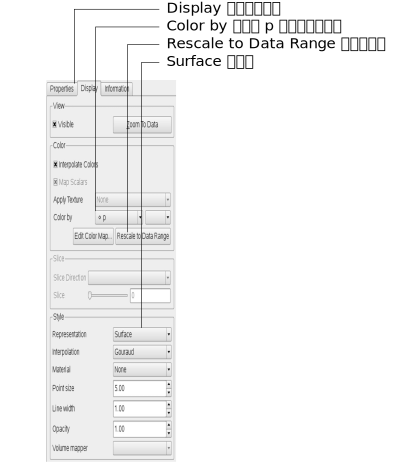
\includegraphics{fig-2-4}
 \caption{キャビティケースでの圧力等圧線の描画}
 \label{fig:2.4}
\end{figure}


\begin{figure}[ht]
 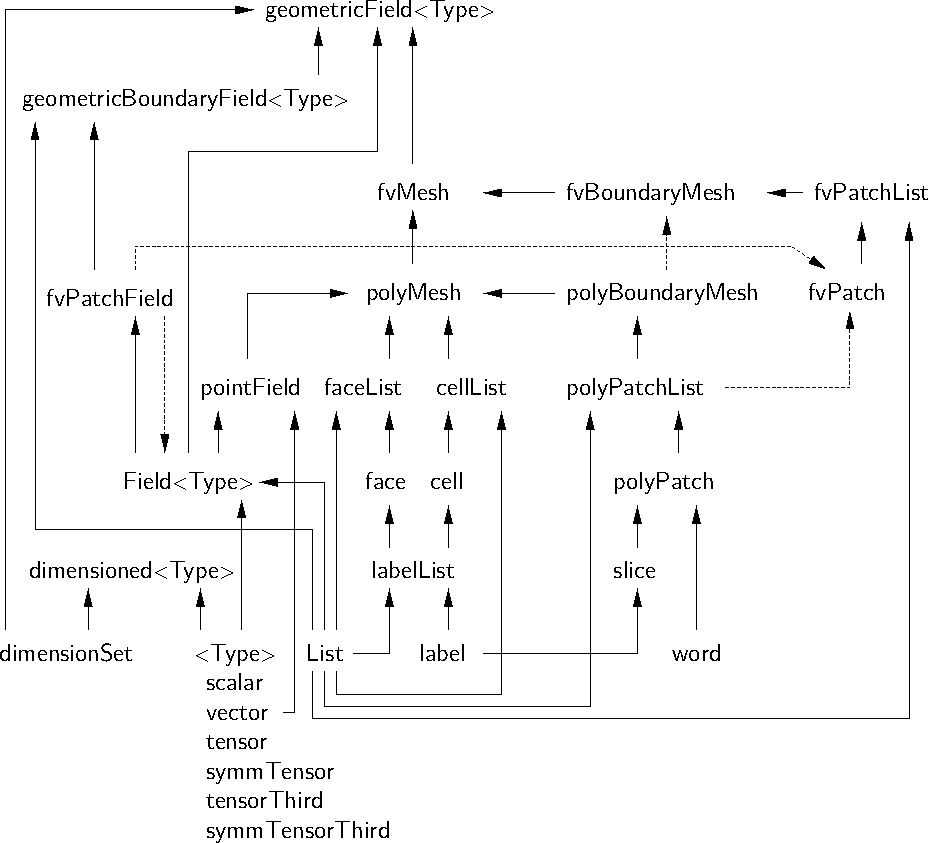
\includegraphics{fig-2-5}
 \caption{キャビティケースでの圧力}
 \label{fig:2.5}
\end{figure}


\subsubsection{ベクトルプロット}
\label{sssec:2.1.4.2}
流速ベクトルを描画する前に,先に作成した断面やコンタなどの
他のモジュールは不要なので取り除きましょう.
\PVwindow{Pipeline Browser}でそれらのモジュールを選択し,
Properties PanelのDeleteをクリックして削除するか,
\PVwindow{Pipeline Browser}で目の形のボタンをクリックして
それらのモジュールを非表示にします.

各格子の中心におけるベクトルグラフを作成することにしましょう.
まず,\autoref{sssec:6.1.7.1}に述べるように
格子の中心のデータのみに絞り込みます.
\PVwindow{Pipeline Browser}上で強調表示されている
cavity.OpenFOAMのモジュールを選択し,
Filter $\rightarrow$ AlphabeticalメニューからCell Centersを選択してApplyをクリックします.

\PVwindow{Pipeline Browser}でCentersが強調表示された状態で,
Filter $\rightarrow$ AlphabeticalメニューからGlyphを選択します.
\autoref{fig:2.6}のような\PVpanel{Properties}ウィンドウが表示されます.
この\PVpanel{Properties}パネルの\PVkeyword{vectors}メニューでは,
ベクトル場は速度のみなので,速度場\OFkeyword{U}が自動的に選択されています.
\PVkeyword{Scale Mode}は速度の\PVkeyword{Vector Magnitude}が初期値として選択されていますが,
領域全体を通る速度の様子を見るために,\PVkeyword{off}を選択し,
\PVentry{Set Scale Factor}に0.005をにします.
\PVbutton{Apply}をクリックするとベクトルが表示されますが,単色,例えば白になっているでしょう.
通常は\PVpanel{Display}パネルで\PVkeyword{Color by U}を選択して速度に応じた色付けをします.
\PVkeyword{Edit Color Map}の中で\PVentry{Show Color Legend}を選択し,
速度の凡例を表示させましょう.出力結果は\autoref{fig:2.7}のようになります.
\index{Color Legend@\PVwindow{Color Legend}!ウィンドウ}%
\index{ウィンドウ!Color Legend@\PVwindow{Color Legend}}%
\PVwindow{Color Legend}(凡例)にはTimes Romanフォントが使用され,
\PVentry{Automatic Label Format}を解除して\PVentry{Label Format}テキストボックスに
\verb|%-#6.2f|を入力することで二つの有効数字でラベルを固定しています.
背景色は,\autoref{sssec:6.1.5.1}で述べるように,
\PVkeyword{View Settings}の\PVpanel{General}パネルで白に設定されています.

左右の壁において,ベトルが壁面を通り抜けるように見えていることに注意してください.
しかし,さらによく調べると,この壁に垂直な方向を向いている速度は$0$であることがわかります.
この少し混乱する状態は,スケーリングが\PVkeyword{off}で速度が$0$のとき,
\OFthirdparty{ParaView}は$x$方向のベクトルで表示するということに起因します.


\begin{figure}[ht]
 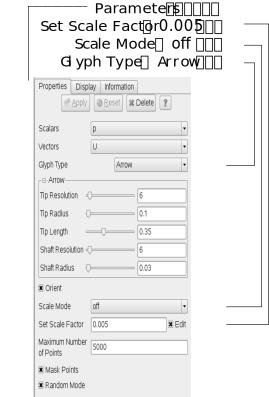
\includegraphics{fig-2-6}
 \caption{Glyphフィルタのパラメータパネル}
 \label{fig:2.6}
\end{figure}


\begin{figure}[ht]
 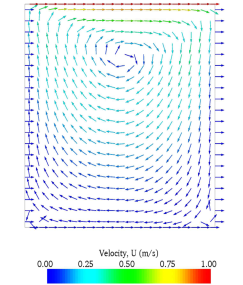
\includegraphics{fig-2-7}
 \caption{キャビティケースの速度}
 \label{fig:2.7}
\end{figure}


\subsubsection{流線プロット}
\label{sssec:2.1.4.3}
\OFthirdparty{ParaView}で後処理を続ける前に,
上述のベクトルプロットのモジュールは不要なので削除しましょう.
そうしたら,\autoref{ssec:6.1.8}の記述のように流速の流線をプロットしましょう.

\PVwindow{Pipeline Browser}で\texttt{cavity.OpenFOAM}モジュールをハイライトした状態で,
\PVmenu{Filter}メニューから\PVfilter{Stream Tracer}を選択し,\PVbutton{Apply}をクリックします.
そうすると,\autoref{fig:2.8}に示すように
\PVpanel{Propaties}ウィンドウが現れます.
\PVentry{Seed}の点は,ジオメトリの中心を垂直に通って,
\PVkeyword{Line Sourse}に沿うように (例えば$(0.05, 0, 0.005)$から
$(0.05, 0.1, 0.005)$まで) 指定しましょう.
このガイドに掲載した図では\PVentry{Point Resolution}を21に,
\PVentry{Max Propagation}を\PVkeyword{Length}で0.5に,
\PVentry{Initial Step Length}を\PVkeyword{Cell Length}で0.01に,
\PVentry{Integration Direction}を\PVkeyword{BOTH}という設定を行いました.
また,\PVkeyword{Runge-Kutta 2} \PVentry{Integrator Type}は
デフォルトパラメータで使いました.

\PVbutton{Apply}をクリックすると,トレーサが生成されます.
そこで\PVmenu{Filter}メニューから\PVkeyword{Tubes}を選択することで,
高品質の流線図を作ることができます.
このレポートでは,次の設定を使いました.
\PVentry{Num.\ sides}を20,\PVentry{Radius}を0.003,\PVentry{Radius factor}を10にしました.
\PVbutton{Accept}を押すことで,\autoref{fig:2.9}ができます.


\begin{figure}[ht]
 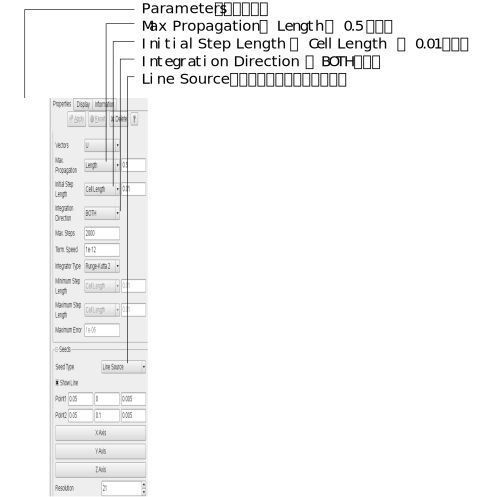
\includegraphics{fig-2-8}
 \caption{Stream Tracerフィルタのパラメータパネル}
 \label{fig:2.8}
\end{figure}


\begin{figure}[ht]
 \includegraphics{fig-2-9}
 \caption{キャビティケースの流線}
 \label{fig:2.9}
\end{figure}


\subsection{メッシュの解像度を増やす}
\label{ssec:2.1.5}
\index{メッシュ!かいぞうど@解像度}%
メッシュの解像度を各々の方向で2倍に増やします.
問題の初期条件として使うために,
粗いメッシュでの結果を,細かいメッシュ上に写像します.
そして,細かいメッシュの解を粗いメッシュの解と比較します.

\subsubsection{既存ケースを用いた新しいケースの作成}
\label{sssec:2.1.5.1}
\OFcase{cavity}をコピーし,
修正することで解析ケース\OFcase{cavityFine}を作成します.
まず\OFpath{cavity}と同じ階層に新しいディレクトリを作成します.
\begin{OFverbatim}[terminal]
cd $FOAM_RUN/tutorials/incompressible/icoFoam
mkdir cavityFine
\end{OFverbatim}%$
基本となる解析ケース\OFpath{cavity}の内容を
解析ケース\OFpath{cavityFine}にコピーし,
\OFpath{cavityFine}に移動します.
\begin{OFverbatim}[terminal]
cp -r cavity/constant cavityFine
cp -r cavity/system cavityFine
cd cavityFine
\end{OFverbatim}

\subsubsection{細かいメッシュの作成}
\label{sssec:2.1.5.2}
\OFtool{blockMesh}を使って計算格子数を増やしましょう.
\OFdictionary{blockMeshDict}ファイルをエディタで開き,
ブロックに関する記述を修正します.
ブロックを特定するには
\index{blocks@\OFkeyword{blocks}!キーワード}%
\index{キーワード!blocks@\OFkeyword{blocks}}%
\OFkeyword{blocks}というキーワードを用いましょう.
ブロック定義の対称性に関しては\autoref{sssec:5.3.1.3}で詳しく述べるので,
ここではhexが最初の頂点リストで,
各方向の計算格子の番号リストがあることを知ればよいでしょう.
これは,先の\OFcase{cavity}ケースでは\texttt{(20 20 1)}になっています.
これを\texttt{(40 40 1)}に変え,保存します.
ここで\OFtool{blockMesh}を実効することで新しい,
より細かいメッシュを生成することができます.

\subsubsection{粗いメッシュの結果を細かなメッシュにマッピングする}
\label{sssec:2.1.5.3}
\index{mapFields@\OFtool{mapFields}!ユーティリティ}%
\index{ユーティリティ!mapFields@\OFtool{mapFields}}%
\OFtool{mapFields}ユーティリティは,他のジオメトリの対応するフィールドの上へ
与えられたジオメトリに関した一つ以上のフィールドをマッピングします.
本チュートリアルの例では,入力フィールドと求める結果のフィールド両方の
ジオメトリ・境界の種類・境界条件が同一であるので,
フィールドは『首尾一貫している』と考えられます.
この例で\OFtool{mapFields}を実行するとき,
\texttt{-consistent}コマンドラインオプションを使います.

mapFields mapsのフィールドデータは,
目的ケース(すなわち結果が図にされている)の
\index{controlDict@\OFdictionary{controlDict}!ディクショナリ}%
\index{ディクショナリ!controlDict@\OFdictionary{controlDict}}%
\OFdictionary{controlDict}内の
startFrom/startTimeで指定される時間ディレクトリから読まれます.
この例では,\OFcase{cavityFine}ケースの細かいメッシュ上に\OFcase{cavity}ケースから
粗いメッシュの最終結果をマッピングしましょう.
これらの結果が\OFpath{cavity}の\OFpath{0.5}のディレクトリに格納されているので,
startTimeを\OFdictionary{controlDict}ディクショナリで$0.5\unit{s}$に,
startFromをstartTimeにセットします.これらの変更を保存しましょう.

\OFtool{mapFields}を実行する準備ができました.
\texttt{mapFields -help}と打ち込むと\OFtool{mapFields}の実行には入力ケースの
ディレクトリを指定する必要があることがわかります.
\texttt{-consistent}オプションを使うので,
次のようにユーティリティは\OFpath{cavityFine}ディレクトリから実行される.
\begin{OFverbatim}[terminal]
mapFields ../cavity -consistent
\end{OFverbatim}
\OFtool{mapFields}が実行され次のように出力されるでしょう.
\begin{OFverbatim}[baselinestretch=0.8, weight=\small]
Source: ".." "cavity"
Target: "." "cavityFine"

Create databases as time

Source time: 0.5
Target time: 0.5
Create meshes

Source mesh size: 400   Target mesh size: 1600

Consistently creating and mapping fields for time 0.5

    interpolating p
    interpolating U

End
\end{OFverbatim}

\subsubsection{設定の調整}
\label{sssec:2.1.5.4}
さて,全てのセルの寸法が半分になったので,
$1$より小さいクーラン数を維持するためには\autoref{sssec:2.1.1.4}で述べるように
時間ステップを半分にしなければいけません.
deltaTを\OFdictionary{controlDict}ディクショナリにて$0.0025\unit{s}$に設定しましょう.
いままでは,フィールドデータを固定のステップ回数のもとでの時間間隔で
出力する方法を示してきましたが,
今回は固定の計算時間でデータ出力を指定する方法を示してみましょう.
\OFdictionary{controlDict}の\OFkeyword{writeControl}キーワード下において,
\index{timeStep@\OFkeyword{timeStep}!キーワードエントリ}%
\index{キーワードエントリ!timeStep@\OFkeyword{timeStep}}%
\OFkeyword{timeStep}エントリで固定のステップ回数で出力する代わりに,
\index{runTime@\OFkeyword{runTime}!キーワードエントリ}%
\index{キーワードエントリ!runTime@\OFkeyword{runTime}}%
\OFkeyword{runTime}を使って固定の計算時間を指定して結果を出力することができます.

このケースでは0.1ごとの出力を指定します.
したがって,\OFkeyword{writeControl}を\OFkeyword{runTime}に,
\index{writeInterval@\OFkeyword{writeInterval}!キーワード}%
\index{キーワード!writeInterval@\OFkeyword{writeInterval}}%
\OFkeyword{writeInterval}を0.1に設定しましょう.このようにすることで,
ケースは粗いメッシュでの解を入力条件として計算をはじめるので,
定常状態に収束するには適切な短い時間だけ動かせばよいのです.
したがって,\OFkeyword{endTime}は$0.7\unit{s}$でよいでしょう.
これらの設定が正しいことを確認し,ケースを保存しましょう.

\subsubsection{バックグラウンドプロセスとしてコードを動かす}
\label{sssec:2.1.5.5}
\OFtool{icoForm}をバックグラウンドプロセスとして動かしてみて,
最終的な結果を後で見ることができるように\OFpath{log}ファイルに出力しましょう.
\OFpath{cavitiyFine}ディレクトリにおいて次のコマンドを実行してください.
\begin{OFverbatim}[terminal]
icoFoam > log &
cat log
\end{OFverbatim}

\subsubsection{精密なメッシュによるベクトルプロット}
\label{sssec:2.1.5.6}
各々の新しいケースは本質的には単なるPipeline Browserに現れる
他のモジュールであるので,
\OFthirdparty{ParaView}で同時に複数のケースを開くことができます.
若干不便なことには,\OFthirdparty{ParaView}で新しいケースを開けるときには,
選ばれたデータが拡張子を含むファイル名である必要があります.
しかし,OpenFOAMにおいて,
各々のケースは特定のディレクトリ構造の中に拡張子なしで
複数のファイルに保存されます.
解決方法として,\OFtool{paraFoam}スクリプトが自動的に拡張子
\OFpath{.OpenFOAM}が付いたダミーファイルを作成することになっています.
それゆえに,\OFcase{cavity}ケースモジュールは
\texttt{cavity.OpenFOAM}と名づけられます.

\OFthirdparty{ParaView}内から他のケースディレクトリを開けたいならば,
そのようなダミーファイルを作成する必要があります.
たとえば,\OFcase{cavityFine}ケースを読み込むには,
コマンドプロンプトで次のようにタイプしてファイルを作成します.
\begin{OFverbatim}[terminal]
cd $FOAM_RUN/tutorials/incompressible/icoFoam
touch cavityFine/cavityFine.OpenFOAM
\end{OFverbatim}%$

こうしてFileメニューからOpen Dataを選んでディレクトリツリーをたどり,\break
\texttt{cavityFine.OpenFOAM}を選ぶことで,
cavityFineケースを\OFthirdparty{ParaView}に読み込めるようになりました.
さて,\OFthirdparty{ParaView}で精密なメッシュの結果の
ベクトルプロットを作ることができます.
同時に両方のケースのglyphを見られるようににすることによって,
\OFcase{cavityFine}ケースのプロットを\OFcase{cavity}ケースと比較することができます.


\begin{figure}[ht]
 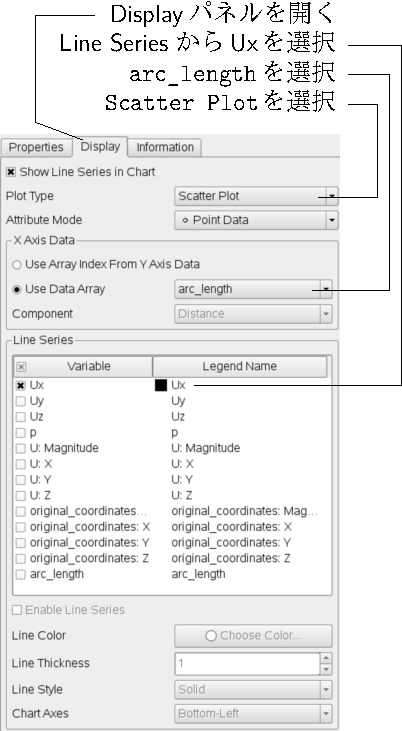
\includegraphics{fig-2-10}
 \caption{グラフ作図のためのフィールド選択}
 \label{fig:2.10}
\end{figure}


\subsubsection{グラフを描く}
\label{sssec:2.1.5.7}
OpenFOAMは,速度のスカラ値を抽出して2次元のグラフに
描画したい場合のデータの取り扱いに長けています.
データを操作するための特別なユーティリティが多数あり,
単純な計算を
\index{foamCalc@\OFtool{foamCalc}!ユーティリティ}%
\index{ユーティリティ!foamCalc@\OFtool{foamCalc}}%
\OFtool{foamCalc}によって組み合わせることができます.
次のようにユーティリティを指定して実行します.
\begin{OFverbatim}[terminal]
foamCalc <calcType> <fieldName1 ... fieldNameN>
\end{OFverbatim}
処理を規定する\texttt{<calcType>}には\texttt{addSubtract},
\texttt{randomise},\texttt{div},\texttt{components},\texttt{mag},
\texttt{magGrad},\texttt{magSqr},\texttt{interpolate}を指定することができます.
\texttt{<calcType>}のリストを見るには,
意図的に無効な処理を要求することでエラーメッセージとともに見ることができます.
\begin{OFverbatim}[baselinestretch=0.8, weight=\small]
>> foamCalc xxxx
Selecting calcType xxxx
unknown calcType type xxxx, constructor not in hash table
Valid calcType selections are:

8
(
randomise
magSqr
magGrad
addSubtract
div
mag
interpolate
components
)
\end{OFverbatim}

\OFkeyword{components}および\OFkeyword{mag}の\OFkeyword{calcType}はスカラ速度を計測するのに有用です.
ケースにて ``\texttt{foamCalc components U}'' を動かすと,
各時刻のディレクトリから速度のベクトル場を読み込み,
各ディレクトリに各軸方向成分のスカラ場
\OFkeyword{Ux},\OFkeyword{Uy},\OFkeyword{Uz}を書き出します.
同様に ``\texttt{foamCalc mag U}'' とは各時刻のディレクトリに
スカラ場\OFkeyword{magU}を書き込みます.

\OFtool{foamCalc}は\OFcase{cavity}と
\OFcase{cavityFine}のどちらに対しても実行することができます.
例えば\OFcase{cavity}に対しては,
以下のように\OFpath{cavity}ディレクトリに移動して\OFtool{foamCalc}を実行します.
\begin{OFverbatim}[terminal]
cd $FOAM_RUN/tutorials/incompressible/icoFoam/cavity
foamCalc components U
\end{OFverbatim}%$
それぞれの成分が\OFthirdparty{ParaView}内でグラフとして描画されます.
簡単に,早く,しかもラベル付けや形式化の調整ができるので,
とても高性能な出力を表示ができます.
しかしながら,出版用にグラフを作成するならばgnuplotやGrace/xmgrなどの
専用のグラフ描画ソフトを使って生データから作画するのがよいでしょう.
これを行うには,\autoref{sec:6.5}や\autoref{ssec:2.2.3}で述べる
\OFtool{sample}ユーティリティを使うとよいでしょう.

描画をする前に,新しく生成された\OFkeyword{Ux},\OFkeyword{Uy},\OFkeyword{Uz}のデータを
\OFthirdparty{ParaView}に読み込ませる必要があります.
これには,\texttt{cavity.OpenFOAM}モジュールのPropertiesパネルの上部にある
Refresh Timesをクリックします.
これにより,\OFthirdparty{ParaView}に新しいフィールドが読み込まれ,
Volume Fieldsウィンドウに現れます.
新しいフィールドを選択し,変更が適用されたことを確認します.
つまり,必要ならApplyを再度クリックします.
また,Mesh Partsパネルで境界領域が選択されているならば,
境界部分のデータ補間が不適切に行われています.
したがって,Mesh Partsパネルで,
\OFpatch{movingwall}や\OFpatch{fixedwall},\OFpatch{frontAndBack}といった
パッチの選択を解除して,変更を適用します.

さて,\OFthirdparty{ParaView}でグラフを表示してみましょう.
まずは描画したいモジュールを選択し,
\index{Plot Over Line@\PVfilter{Plot Over Line}!メニューエントリ}%
\index{メニューエントリ!Plot Over Line@\PVfilter{Plot Over Line}}%
\PVfilter{Plot Over Line}フィルタを\PVmenu{Filter} $\rightarrow$ \PVmenu{Data Analisys}から選択します.
\PVwindow{3D View}ウィンドウの下または横に新しい\PVwindow{XY Plot}ウィンドウが開きます.
\PVpanel{Properties}ウィンドウで線の終点を指定すると
Plobelineモジュールが作成されます.
この例ではPoint1を$(0.05, 0, 0.005)$,
Point2を$(0.05, 0.1, 0.005)$と指定して線を領域の中心の真上におきます.
Resolutionは100まで設定できます.

\PVbutton{Apply}をクリックすると\PVwindow{XY Plot}ウィンドウにグラフが描画されます.
\PVpanel{Display}パネルで,
\index{Attribute Mode@\PVmenu{Attribute Mode}!メニュー}%
\index{メニュー!Attribute Mode@\PVmenu{Attribute Mode}}%
\PVmenu{Attribute Mode}を\PVkeyword{Point Data}に設定します.
\PVkeyword{Use Data Array}オプションを\PVkeyword{X Axis Data}にし,
\verb|arc_length|オプションを加えて,
グラフの$x$軸データがキャビティの底からの距離になるようにできます.

\PVpanel{Display}ウィンドウの\PVpanel{Line Series}パネルから
表示するデータを選択することができます.
表示されているスカラ場のリストから,
ベクトルの大きさや成分を初期値とすることもできます.
つまり,\OFkeyword{Ux}を\OFtool{foamCalc}から計算する必要はありません.
それでも,\OFkeyword{Ux}以外の系列の選択はすべて解除しましょう.
選択した系列の上の四角形の色が線の色です.
この上でダブルクリックをすれば簡単に変更することができます.

グラフの体裁を整えるには,\PVpanel{Line Series}パネルの下にある設定,
\PVkeyword{Line Color},\PVkeyword{Line Thickness},\PVkeyword{Line Style},
\PVkeyword{Marker Style},そして\PVkeyword{Chart Axes}を変更します.

また,\PVwindow{XY Plot}の左上にあるボタンをクリックすることもできます.
例えば,3番目のボタンでは,それぞれの軸のタイトルや凡例などを設定する
\PVentry{View Settings}を制御することができます.
また,軸のタイトルのフォント,色,配置,
値の範囲や線形・対数表示など,様々な設定を行うことができます.

\autoref{fig:2.11}は\OFthirdparty{ParaView}によって作画された図です.
望みどおりのグラフが作成できます.
\autoref{fig:2.11}は軸のオプションとして
Standard type of Notation,Specify Axis Rangeを選択し,
フォントはSans Serifの12ポイントです.
このグラフは点で表示していますが,
\PVpanel{Display}ウィンドウで
\index{Enable Line Series@\PVbutton{Enable Line Series}!ボタン}%
\index{ボタン!Enable Line Series@\PVbutton{Enable Line Series}}%
\PVbutton{Enable Line Series}ボタンを
有効にすれば線で表示できます.
注:もしこのボタンが,グレー表示で無効の状態になっていたら,
\PVpanel{Line Series}パネルでどれか変数を選択すれば有効になります.
\PVbutton{Enable Line Series}ボタンを選択しておけば,
\index{Line Style@\PVmenu{Line Style}!メニュー}%
\index{メニュー!Line Style@\PVmenu{Line Style}}%
\PVmenu{Line Style}や
\index{Marker Style@\PVmenu{Marker Style}!メニュー}%
\index{メニュー!Marker Style@\PVmenu{Marker Style}}%
\PVmenu{Marker Style}もユーザの好みで調整できます.


\begin{figure}[ht]
 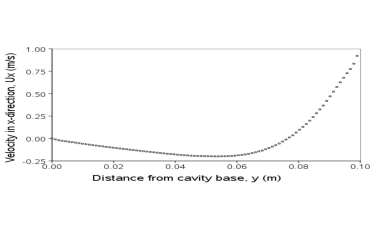
\includegraphics{fig-2-11}
 \caption{\OFtool{paraFoam}でのグラフ作図}
 \label{fig:2.11}
\end{figure}


\subsection{勾配メッシュ}
\label{ssec:2.1.6}
解の誤差は,正しい解の形と選択した数値スキームで想定される形とが
大きく異なる領域で出ます.
例えば,数セルにわたる変数の線形変化に基づく数値スキームは,
正しい解自体が線形の場合にしか正確な解を導くことができません.
例えば勾配の変化が最も大きいところのような正しい解が
線形から一番大きく外れる領域で誤差は最も大きくなります.
セルの大きさに従って,誤差は減少します.

どんな問題も取りかかる前に解の概形の直感的予測ができるといいです.
次に,誤差が最も大きくなるところを予測し,メッシュ幅に勾配をつけ,
最も小さいセルがこれらの領域にくるようにします.
キャビティの場合,壁の近くで速度の大きい変化があることを予想できるので,
チュートリアルのこの部分では,メッシュがこの領域で,
より小さくなるように勾配付けします.
同じ数のセルを使用することによって,
コンピュータの負荷をあまり増加させずに,より精度を上げられます.

lid-drivenキャビティ問題のために壁に向かって勾配を付けた
$20 \times 20$セルのメッシュを作り,
\autoref{sssec:2.1.5.2}の細かいメッシュの結果を初期条件として
勾配付けされたメッシュに適用しましょう.
そして,勾配付けされたメッシュの結果を前のメッシュの結果と
比較してみましょう.
\index{blockMeshDict@\OFdictionary{blockMeshDict}!ディクショナリ}%
\index{ディクショナリ!blockMeshDict@\OFdictionary{blockMeshDict}}%
\OFdictionary{blockMeshDict}ディクショナリの書換えはとても重要であるので,
チュートリアルのこの部分を使ったケース (\OFpath{cavityGrade}) は
\OFpath{\$FOAM\_RUN/tutorials/incompressible/icoFoam}ディレクトリに入れておきました.

\subsubsection{勾配メッシュの作成}
\label{sssec:2.1.6.1}
ここで,四つの異なるメッシュ間隔の計算メッシュが計算領域の
上下左右のブロックに必要となります.
このメッシュのブロック構造を\autoref{fig:2.12}に示します.


\begin{figure}[ht]
 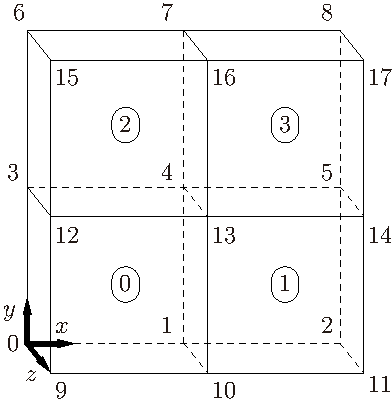
\includegraphics{fig-2-12}
 \caption{キャビティケースの勾配メッシュのブロック構造(ブロック番号)}
 \label{fig:2.12}
\end{figure}


\OFpath{cavityGrade}の\OFpath{constant/polyMesh}サブディレクトリで
\OFdictionary{blockMeshDict}ファイルを見ることができます.
念のため\OFdictionary{blockMeshDict}の重要な要素を以下に述べます.
それぞれのブロックは$x$方向,$y$方向に10セルを有し,
もっとも大きなセルともっとも小さなセルとの大きさの比は2です.
\begin{OFverbatim}[file, linenum=17]
/*--------------------------------*- C++ -*----------------------------------*\
| =========                 |                                                 |
| \\      /  F ield         | OpenFOAM: The Open Source CFD Toolbox           |
|  \\    /   O peration     | Version:  2.0.0                                 |
|   \\  /    A nd           | Web:      www.OpenFOAM.com                      |
|    \\/     M anipulation  |                                                 |
\*---------------------------------------------------------------------------*/
FoamFile
{
    version     2.0;
    format      ascii;
    class       dictionary;
    object      blockMeshDict;
}
// * * * * * * * * * * * * * * * * * * * * * * * * * * * * * * * * * * * * * //

convertToMeters 0.1;

vertices        
(
    (0 0 0)
    (0.5 0 0)
    (1 0 0)
    (0 0.5 0)
    (0.5 0.5 0)
    (1 0.5 0)
    (0 1 0)
    (0.5 1 0)
    (1 1 0)
    (0 0 0.1)
    (0.5 0 0.1)
    (1 0 0.1)
    (0 0.5 0.1)
    (0.5 0.5 0.1)
    (1 0.5 0.1)
    (0 1 0.1)
    (0.5 1 0.1)
    (1 1 0.1)
);

blocks          
(
    hex (0 1 4 3 9 10 13 12) (10 10 1) simpleGrading (2 2 1)
    hex (1 2 5 4 10 11 14 13) (10 10 1) simpleGrading (0.5 2 1)
    hex (3 4 7 6 12 13 16 15) (10 10 1) simpleGrading (2 0.5 1)
    hex (4 5 8 7 13 14 17 16) (10 10 1) simpleGrading (0.5 0.5 1)
);

edges           
(
);

boundary
(
    movingWall
    {
        type wall;
        faces
        (
            (6 15 16 7)
            (7 16 17 8)
        );
    }
    fixedWalls
    {
        type wall;
        faces
        (
            (3 12 15 6)
            (0 9 12 3)
            (0 1 10 9)
            (1 2 11 10)
            (2 5 14 11)
            (5 8 17 14)
        );
    }
    frontAndBack
    {
        type empty;
        faces
        (
            (0 3 4 1)
            (1 4 5 2)
            (3 6 7 4)
            (4 7 8 5)
            (9 10 13 12)
            (10 11 14 13)
            (12 13 16 15)
            (13 14 17 16)
        );
    }
);

mergePatchPairs
(
);

// ************************************************************************* //
\end{OFverbatim}
いったんこのケースの\OFdictionary{blockMeshDict}ファイルを理解しておけば,
後はコマンドラインから\OFtool{blockMesh}を実行できます.
\autoref{ssec:2.1.2}に示した\OFtool{paraFoam}を使用することで
勾配付けされたメッシュを見ることができます.

\subsubsection{計算時間,時間ステップの変更}
\label{sssec:2.1.6.2}
もっとも速い速度と小さいセルが上蓋に面することになり,
したがって,\autoref{sssec:2.1.1.4}で示したように,
もっとも高いクーラン数が上蓋に面するセルに生じます.
このようなことから上蓋に面するセルの大きさを見積もることは,
本ケースにて適当な時間ステップを計算する上で有効です.

一様でないメッシュ勾配を使用している場合,
\index{blockMesh@\OFtool{blockMesh}!ユーティリティ}%
\index{ユーティリティ!blockMesh@\OFtool{blockMesh}}%
\OFtool{blockMesh}は形状に関する数列をもちいてセルの大きさを算出します.
長さ$l$に沿って,最初と最後のセルとの間に,
比$R$の$n$個の計算セルが必要であるならば,
もっとも小さいセルの大きさは,次のように与えられます.
\begin{align}
 \label{eq:2.5}
  \Delta x_{\mathrm{s}} = l\frac{r - 1}{\alpha r - 1}
\end{align}
ここで,$r$はあるセルの大きさとその隣のセルの大きさとの比であり,
次式で表されます.
\begin{align}
 \label{eq:2.6}
  r = R^{\frac{1}{n-1}}
\end{align}
そして,
\begin{align}
 \label{eq:2.7}
  \alpha =
  \begin{cases}
   R & \text{for}\ R > 1, \\
   1 - r^{-1} + r^{-1} & \text{for}\ R < 1.
  \end{cases}
\end{align}
\OFcase{cavityGrade}ケースにおいては,各方向のセルの数は$10$であり,
もっとも大きなセルと小さなセルとの比は$2$,
ブロックの縦横は$0.05\unit{m}$です.
したがって,もっとも小さなセルサイズは$3.45\unit{mm}$となります.
\autoref{eq:2.2} から時間ステップは,クラーン数を$1$以下に抑えるために
$3.45\unit{ms}$以下にしなければなりません.
有意な解析結果を得るためには,
時間ステップ\OFkeyword{deltaT}を$2.5\unit{ms}$まで短くし,
\OFkeyword{writeInterval}を40とします.
これより解析結果は$0.1\unit{s}$ごとに書き出されることとなります.

このように,各設定に対応したファイルを編集することにより,
ケースディクショナリの各種条件を変更することができます.
ここで時間ないし計算経過の書き出しを操作したいならば,
\OFpath{/cavityGrade/system/controlDict}ファイル内に
それらのパラメータは納められており,
任意のエディタでこのファイルを開くことができます.
先に述べたように,計算を収束させるための保証として,
このケースでは時間ステップ\OFkeyword{deltaT}は\texttt{0.25e-3}に,
\OFkeyword{writeInterval}は40とします.

\OFkeyword{startTime}はその\OFcase{cavityFine}ケースの最終的な条件,
すなわち$0.7$に設定される必要があります.
\OFcase{cavity}と\OFcase{cavityFine}が規定された実行時間の中でよく収束させるためには,
\OFcase{cavityGrade}ケースのための実行時間を$0.1\unit{s}$に設定,
すなわち\OFkeyword{endTime}を0.8とします.

\subsubsection{解析場のマッピング}
\label{sssec:2.1.6.3}
\autoref{sssec:2.1.5.3}にあるように
\index{mapFields@\OFtool{mapFields}!ユーティリティ}%
\index{ユーティリティ!mapFields@\OFtool{mapFields}}%
\OFtool{mapFields}を使用して,
\OFcase{cavityFine}ケースの最終的な結果を
\OFcase{cavityGrade}ケースのメッシュにマッピングします.
以下のように\OFpath{cavityGrade}ディレクトリに入り,
\OFtool{mapFields}を実行してください.
\begin{OFverbatim}[terminal]
cd $FOAM_RUN/tutorials/incompressible/icoFoam/cavityGrade
mapFields ../cavityFine -consistent
\end{OFverbatim}%$
今度は,ケースディレクトリから\OFtool{icoFoam}を実行します.
そして,ランタイム情報をモニタリングします.
そして,このケースの完全に収束した結果を見て,
以前に\autoref{sssec:2.1.5.6}と\autoref{sssec:2.1.5.7}で説明した
後処理ツールを使って他の結果と比較します.


\subsection{レイノルズ数の増大}
\label{ssec:2.1.7}
これまで解いたケースはレイノルズ数が$10$でした.
これは大変に低い条件であり,
したがってキャビティの底部中央に小さな二次渦を伴うのみで,
迅速に安定解を導くことができました.
しかし,ここでレイノルズ数を$100$に上げると,
収束解を得るのにより長い時間を要することになります.
そこで\OFcase{cavity}ケースのメッシュを初期条件として使用することとします.
\OFpath{cavity}ケースディレクトリを\OFpath{cavityHighRe}という名前でコピーします.
\begin{OFverbatim}[terminal]
cd $FOAM_RUN/tutorials/incompressible/icoFoam
cp -r cavity cavityHighRe
\end{OFverbatim}%$

\subsubsection{後処理}
\label{sssec:2.1.7.1}
\OFpath{cavityHighRe}ケースに入り,
\index{transportProperties@\OFdictionary{transportProperties}!ディクショナリ}%
\index{ディクショナリ!transportProperties@\OFdictionary{transportProperties}}%
\OFdictionary{transportProperties}ディクショナリを編集します.
レイノルズ数を10倍に増加させるためには,
動粘性係数を10分の1まで減らす必要があります(例えば10から).
これで\OFcase{cavity}ケースの実行結果から
\index{リスタート}%
リスタートして,このケースを実行できます.
これを実行するために,\OFkeyword{startFrom}キーワードを
\index{latestTime@\OFkeyword{latestTime}!キーワードエントリ}%
\index{キーワードエントリ!latestTime@\OFkeyword{latestTime}}%
\OFkeyword{latestTime}に
オプションを切り替えることにより,
\OFtool{icoFoam}は,最新の時間ディレクトリを初期データとして使用します(例えば0.5).
\OFkeyword{endTime}は$2\unit{s}$に設定し,本ケースを保存します.

\subsubsection{コードの実行}
\label{sssec:2.1.7.2}
まずはケースディレクトリから\OFtool{icoFoam}を実行し,ランタイム情報を見ます.
バックグラウンドでジョブを実行するときには,以下のUNIXコマンドが便利です.
\begin{description}
 \item[\texttt{nohup}]
            ユーザがログアウト後も稼働し続けるコマンド
 \item[\texttt{nice}]
            カーネル・スケジューラのジョブの優先順位を変えるコマンド.
            $-20$が最優先で,$19$は最も低い優先度.
\end{description}
これらのコマンドは,
例えば,ユーザがリモートマシンでケースを実行できるよう設定し,
頻繁にモニタしなくてもいいような場合,
リモートマシンではケース実行をあまり優先させたくないでしょうが,
そのような場合に便利です.
その場合,ユーザは\texttt{nohup}コマンドで稼働しているリモートマシンを
ログアウトしてジョブを実行し続けることができます.
一方,\texttt{nice}は優先度を19に設定します.
試しに,以下のようにコマンドを実行してみましょう.
\begin{OFverbatim}[terminal]
cd $FOAM_RUN/tutorials/incompressible/icoFoam
nohup nice -n 19 icoFoam > log &
cat log
\end{OFverbatim}%$
お気づきかもしれませんが,前述の解析方法では\OFtool{icoFoam}は,
速度\OFkeyword{U}の計算が止まっても,
それよりもずっと長い間もしくは解析が終わるまで
圧力\OFkeyword{p}の計算をし続けていました.
実際には,\OFtool{icoFoam}がいったん\OFkeyword{U}の計算をやめ,
\OFkeyword{p}の初期残差が\OFdictionary{fvSolution}ディクショナリで
設定された許容値(通常は$10^{-6}$)を下回ると
結果が効率的に収束するので,
フィールド・データをいったん時間ディレクトリに書き出して
計算を止めることができます.
例として,\OFcase{cavityHighRen}ケースの
\index{しゅうそく@収束}%
収束の\OFpath{log}ファイルを以下に示します.
示したとおり,$1.62\unit{s}$後に速度はすでに収束し,
初期の圧力残差は小さくなります.
\OFpath{log}において\verb|No Iterations 0|は,
\OFkeyword{U}の計算が止まったことを示しています.
\begin{OFverbatim}[file, linenum, weight=\footnotesize]

Time = 1.63

Courant Number mean: 0.108642 max: 0.818175
DILUPBiCG:  Solving for Ux, Initial residual = 7.86044e-06, Final residual = 7.86044e-06,
No Iterations 0
DILUPBiCG:  Solving for Uy, Initial residual = 9.4171e-06, Final residual = 9.4171e-06,
No Iterations 0
DICPCG:  Solving for p, Initial residual = 3.54721e-06, Final residual = 7.13506e-07,
No Iterations 4
time step continuity errors : sum local = 6.46788e-09, global = -9.44516e-19,
cumulative = 1.04595e-17
DICPCG:  Solving for p, Initial residual = 2.15824e-06, Final residual = 9.95068e-07,
No Iterations 3
time step continuity errors : sum local = 8.67501e-09, global = 7.54182e-19,
cumulative = 1.12136e-17
ExecutionTime = 1.02 s  ClockTime = 1 s

Time = 1.635

Courant Number mean: 0.108643 max: 0.818176
DILUPBiCG:  Solving for Ux, Initial residual = 7.6728e-06, Final residual = 7.6728e-06,
No Iterations 0
DILUPBiCG:  Solving for Uy, Initial residual = 9.19442e-06, Final residual = 9.19442e-06,
No Iterations 0
DICPCG:  Solving for p, Initial residual = 3.13107e-06, Final residual = 8.60504e-07,
No Iterations 4
time step continuity errors : sum local = 8.15435e-09, global = -5.84817e-20,
cumulative = 1.11552e-17
DICPCG:  Solving for p, Initial residual = 2.16689e-06, Final residual = 5.27197e-07,
No Iterations 14
time step continuity errors : sum local = 3.45666e-09, global = -5.62297e-19,
cumulative = 1.05929e-17
ExecutionTime = 1.02 s  ClockTime = 1 s
\end{OFverbatim}


\subsection{高レイノルズ数流れ}
\label{ssec:2.1.8}
では,\OFtool{paraFoam}による結果を確認し,速度ベクトルを表示してください.
計算領域の角における二次渦が幾分増大していることがわかります.
このようなとき,ユーザは粘性係数を下げることにより
レイノルズ数を増大させた計算ケースを再度実行できます.
渦の数が増加するにともない,より複雑な流れを解くために
当該領域でのメッシュ解像度を上げる必要がでてきます.
さらに,レイノルズ数は収束に要する時間を増加させます.
このような場合,残差をモニタし,解を収束させるために
\OFkeyword{endTime}を延長したほうがよいでしょう.

空間および時間解像度の増加を要することは,
流れが乱流域に移行するという非現実的な状態となり,
解法の安定性の問題が生じることとなります.
もちろん,多くの工学的な問題は
極めて高いレイノルズ数条件となっており,
したがって,乱流挙動を直接解くのに多くのコストを負担することとなり,
実行不可能であります.
そのかわりに,
\index{らんりゅうモデル@乱流モデル!RAS}%
レイノルズ平均シミューレション (RAS) 乱流モデルが
平均流れの挙動を解くのに用いられ,
ゆらぎの統計値が計算されています.
壁関数を伴う標準$k$--$\varepsilon$モデルが
本チュートリアルの上面が移動する
キャビティケース(レイノルズ数$10^{4}$)を解くのに用いられています.
二つの追加変数が解かれています.
それは,
\index{らんりゅう@乱流!うんどうエネルギ@運動エネルギ}%
乱流エネルギ$k$,
\index{らんりゅう@乱流!しょうさん@消散}%
乱流消散速度$\varepsilon$です.
乱流のための追加の方程式およびモデルは\OFtool{pisoFoam}と呼ばれる
OpenFOAMソルバにおいて実行されます.

\subsubsection{前処理}
\label{sssec:2.1.8.1}
\OFpath{\$FOAM\_RUN/tutorials/incompressible/pisoFoam/ras}ディレクトリの
\OFpath{cavity}ケースに移動します.
これまでと同様に,\OFtool{blockMesh}を走らせ,
メッシュを生成します.
壁関数付き標準$k$--$\varepsilon$モデルを用いる場合は,
壁近傍のセルにおける流れがモデル化されることにより,
壁方向へのメッシュ勾配は必ずしも必要ではありません.

OpenFOAMでは,様々な壁関数モデルを利用することができ,
それぞれのパッチの境界条件として設定します.
これにより,壁面ごとに異なる壁関数モデルを適用することが可能になります.
壁関数の選択は,乱流粘性係数$\nu_{\mathrm{t}}$の
ファイル\OFpath{0/nut}で指定します.
\begin{OFverbatim}[file, linenum=17]

dimensions      [0 2 -1 0 0 0 0];

internalField   uniform 0;

boundaryField
{
    movingWall
    {
        type            nutkWallFunction;
        value           uniform 0;
    }
    fixedWalls
    {
        type            nutkWallFunction;
        value           uniform 0;
    }
    frontAndBack
    {
        type            empty;
    }
}


// ************************************************************************* //
\end{OFverbatim}
このケースでは,\OFpatch{movingWall}と\OFpatch{fixedWalls}のパッチに対して
\OFkeyword{nutWallFunction}キーワードエントリで標準的な壁関数を指定しています.
これ以外の壁関数モデルとしては,
粗壁面の壁関数\OFkeyword{nutRoughWallFunction}などがあります.

次に,$k$と$\varepsilon$のファイル (\OFpath{0/k}と\OFpath{0/epsilon}) を開き,
境界条件を確かめます.
壁タイプの境界条件の選択には,
$\varepsilon$については\OFkeyword{epsilonWallFunction}境界条件を,
$k$については\OFkeyword{kqRWallFunction}を指定します.
後者は乱流運動エネルギの表現$k$,$q$,
あるいはレイノルズ応力$R$のいずれにも適用できる一般的な壁関数です.
$k$,$\varepsilon$の初期条件には,
速度変動$\bm{U}'$と
\index{らんりゅう@乱流!ながさスケール@長さスケール}%
乱流長さスケール$l$から推測した値を設定します.
$k$と$\varepsilon$は,これらのパラメタを用いて次式で表されます.
\begin{align}
 \label{eq:2.8}
  k &= \frac{1}{2}\overline{\bm{U}' \cdot \bm{U}'} \\
 \label{eq:2.9}
 \varepsilon &= \frac{C_{\mu}^{0.75}k^{1.5}}{l}
\end{align}
ここで$C_{\mu}$は$k$--$\varepsilon$モデルの定数であり,
その値は$0.09$です.デカルト座標系では$k$は,
\begin{align}
 \label{eq:2.10}
 k = \frac{1}{2}({U_{x}'}^{2} + {U_{y}'}^{2} + {U_{z}'}^{2})
\end{align}
で表されます.各項は$x$,$y$,$z$方向速度ゆらぎ成分です.
ここで,初期乱流が等方的であると仮定します.
例えば,${U_{x}'}^{2} = {U_{y}'}^{2} = {U_{z}'}^{2}$となり,
これら速度は上面速度の$5\unit{\%}$に等しく,
また,乱流長さスケール$l$はボックス幅$0.1\unit{m}$の
$20\unit{\%}$に等しいとすると,次のように表されます.
\begin{align}
 \label{eq:2.11}
 U_{x}' &= U_{y}' = U_{z}' = \frac{5}{100}1\unit{m\,s^{-1}} \\
 \label{eq:2.12}
 \Rightarrow k &= \frac{3}{2}\left(\frac{5}{100}\right)^{2}\unit{m^{2}s^{-2}}
 = 3.75 \times 10^{-3}\unit{m^{2}s^{-2}} \\
 \label{eq:2.13}
 \varepsilon &= \frac{C_{\mu}^{0.75}k^{1.5}}{l}
 \approx 7.65 \times 10^{-4}\unit{m^{2}s^{-3}}
\end{align}
上記のとおり$k$,$\varepsilon$を設定してください.
$U$と$p$に対する初期条件は前と同じように,
それぞれ$(0, 0, 0)$と$0$です.

OpenFOAMで提供されている乱流モデルには,
例えばRASやlarge-edy simulation (LES) のような,
さまざまな手法があります.
ほとんどの非定常ソルバでは,乱流のモデリング手法は
実行時に\OFdictionary{turbulenceProperties}ディクショナリの
\OFkeyword{simulationType}キーワードで選択できます.
このファイルは\OFpath{constant}ディレクトリの中に見つかります.
\begin{OFverbatim}[file, linenum=17]

simulationType  RASModel;


// ************************************************************************* //
\end{OFverbatim}
\OFkeyword{simulationType}の選択肢は
\index{laminar@\OFkeyword{laminar}!キーワードエントリ}%
\index{キーワードエントリ!laminar@\OFkeyword{laminar}}%
\OFkeyword{laminar},
\index{RASModel@\OFkeyword{RASModel}!キーワードエントリ}%
\index{キーワードエントリ!RASModel@\OFkeyword{RASModel}}%
\OFkeyword{RASModel},そして
\index{LESModel@\OFkeyword{LESModel}!キーワードエントリ}%
\index{キーワードエントリ!LESModel@\OFkeyword{LESModel}}%
\OFkeyword{LESModel}です.
このケースで選択されている\OFkeyword{RASModel}の場合,
RASモデリングの選択は
\index{RASProperties@\OFdictionary{RASProperties}!ディクショナリ}%
\index{ディクショナリ!RASProperties@\OFdictionary{RASProperties}}%
\OFpath{RASProperties}ファイルに記述します.
このファイルも同じく\OFpath{constant}ディレクトリにあります.
乱流モデルは\autoref{tbl:3.9}に示されている多くの使用可能なモデルから,
\OFkeyword{RASModel}エントリで選択します.
ここでは,標準$k$--$\varepsilon$モデルである\OFkeyword{kEpsilon}を選択します.
\OFkeyword{turbulence}のスイッチが\OFkeyword{on}になっていることも確認します.
乱流モデルに必要な係数には,それぞれのコードの中でデフォルト値が与えられています.
\index{printCoeffs@\OFkeyword{printCoeffs}!キーワード}%
\index{キーワード!printCoeffs@\OFkeyword{printCoeffs}}%
\OFkeyword{printCoeffs}というオプションのスイッチを\OFkeyword{on}にすると,
実行時に乱流モデルが呼ばれたときに,これらのデフォルト値が標準出力,
すなわちターミナルに出力されるようになります.
これらの係数は,モデル名に\OFkeyword{Coeffs}をつけた名前
(たとえば\OFkeyword{kEpsilon}モデルなら\OFkeyword{kEpsilonCoeffs})
のサブディクショナリとして表示されます.
モデルの係数は,必要に応じて\OFdictionary{RASProperties}ディクショナリに
サブディクショナリを追加(コピー\&ペースト)し,値を適宜調整することで変更することができます.

次いで,
\index{transportProperties@\OFdictionary{transportProperties}!ディクショナリ}%
\index{ディクショナリ!transportProperties@\OFdictionary{transportProperties}}%
\OFdictionary{transportProperties}ディクショナリの層流
\index{ねんせいけいすう@粘性係数!どう@動\jdash}%
動粘性係数を設定します.
レイノルズ数$10^{4}$を実現するために,
\autoref{eq:2.1} のレイノルズ数の定義式に示されるように,
動粘性係数を$10^{-5}\unit{m^{2}s^{-1}}$にする必要があります.

最後に,
\index{controlDict@\OFdictionary{controlDict}!ディクショナリ}%
\index{ディクショナリ!controlDict@\OFdictionary{controlDict}}%
\OFdictionary{controlDict}の\OFkeyword{startTime},
\OFkeyword{stopTime},\OFkeyword{deltaT},
そして\OFkeyword{writeInterval}を設定します.
クーラン数の制限を満たすために\OFkeyword{deltaT}を$0.005\unit{s}$に設定し,
\OFkeyword{endTime}は$10\unit{s}$とします.

\subsubsection{コードの実行}
\label{sssec:2.1.8.2}
ケースディレクトリに入り,ターミナルで\texttt{pisoFoam}とタイプすることで
\OFtool{pisoFoam}を実行します.
粘性が小さいこの計算ケースでは,
移動している上面近傍の境界層は極めて薄く,
そして,上面に面するセルは比較的大きいことから,
上面速度よりもそれらセル中心の流体速度は極めて小さいです.
事実,100時間ステップ後,上面に隣接したセルにおける速度は,
上限である$0.2\unit{m\,s^{-1}}$程度です.
したがって最大クーラン数は$0.2$以上にはなりません.
クーラン数がより$1$に近接するように時間ステップを大きくし,
解析時間を増やすことは理にかなっています.
したがって,\OFkeyword{deltaT}を$0.02\unit{s}$にセットしなおし,
これに伴い,\OFkeyword{startFrom}を\OFkeyword{latestTime}にセットします.
本操作は,\OFtool{pisoFoam}が最新のディレクトリ,例えば\OFpath{10.0},
からスタートデータを読み込むように指示するものです.
\OFkeyword{endTime}は層流条件よりも収束に時間を要するため,
$20\unit{s}$にセットします.
従来どおり計算をリスタートし,解析の収束をモニタします.
解析が進行したら,連続した時間における結果を見てください.
そして解析が安定状態に収束するか,
もしくは周期的に振動しているか確認してください.
後者の場合には,収束は決して起こりませんが,
結果が不正確であるという意味ではありません.


\subsection{ケース形状の変更}
\label{ssec:2.1.9}
計算ケースの形状を変更し,新たな解析を行いたい場合,
新たな解析のスタート条件としてオリジナルの解析の全てないし一部を
保持しておくことは有効でしょう.
しかし,これは少し複雑になります.
なぜなら,オリジナルの解析の物理量が,
新しい解析ケースの物理量と一致しないからです.
しかし,
\index{mapFields@\OFtool{mapFields}!ユーティリティ}%
\index{ユーティリティ!mapFields@\OFtool{mapFields}}%
\OFtool{mapFields}ユーティリティは,形状や境界のタイプもしくは
その両者が不一致な場を位置づけることができます.

例であるように,\OFpath{icoFoam}ディレクトリ内にある
\OFpath{cavityClipped}ケースを開きます.
このケースは,標準的な\OFcase{cavity}ケースからなりますが,
底部右側,長さ$0.04\unit{m}$の正方形を除いたものであり,
\OFdictionary{blockMeshDict}は以下のようになっています.
\begin{OFverbatim}[file, linenum=17]
convertToMeters 0.1;

vertices
(
    (0 0 0)
    (0.6 0 0)
    (0 0.4 0)
    (0.6 0.4 0)
    (1 0.4 0)
    (0 1 0)
    (0.6 1 0)
    (1 1 0)

    (0 0 0.1)
    (0.6 0 0.1)
    (0 0.4 0.1)
    (0.6 0.4 0.1)
    (1 0.4 0.1)
    (0 1 0.1)
    (0.6 1 0.1)
    (1 1 0.1)

);

blocks
(
    hex (0 1 3 2 8 9 11 10) (12 8 1) simpleGrading (1 1 1)
    hex (2 3 6 5 10 11 14 13) (12 12 1) simpleGrading (1 1 1)
    hex (3 4 7 6 11 12 15 14) (8 12 1) simpleGrading (1 1 1)
);

edges
(
);

boundary
(
    lid
    {
        type wall;
        faces
        (
            (5 13 14 6)
            (6 14 15 7)
        );
    }
    fixedWalls
    {
        type wall;
        faces
        (
            (0 8 10 2)
            (2 10 13 5)
            (7 15 12 4)
            (4 12 11 3)
            (3 11 9 1)
            (1 9 8 0)
        );
    }
    frontAndBack
    {
        type empty;
        faces
        (
            (0 2 3 1)
            (2 5 6 3)
            (3 6 7 4)
            (8 9 11 10)
            (10 11 14 13)
            (11 12 15 14)
        );
    }
);

mergePatchPairs
(
);

// ************************************************************************* //
\end{OFverbatim}
\OFtool{blockMesh}を実行してメッシュを生成します.
パッチは\OFcase{cavity}ケースと同様に設定されています.
物理量の適用の過程を明確にするために,
元となるケース\OFcase{cavity}で\OFpatch{movingWall}であった
上側の壁は\OFpatch{lid}という名前に変更されています.

パッチが一致しない場合,
すべての物理量のデータが元のケースからマップされるという保証はありません.
残っているデータは元のケースと同一であるべきです.
したがってマッピングする前に時間のディレクトリに物理量のデータが
存在している必要があります.
\OFdictionary{controlDict}の\OFkeyword{startTime}が$0.5\unit{s}$に設定されているので
\OFcase{cavityClipped}ケースにおけるマッピングは
時刻$0.5\unit{s}$に予定されています.
したがって初期状態の物理量のデータ,
たとえば時刻0からをコピーする必要があります.
\begin{OFverbatim}[terminal]
cd $FOAM_RUN/tutorials/incompressible/icoFoam/cavityClipped
cp -r 0 0.5
\end{OFverbatim}%$

データをマッピングする前に$0.5\unit{s}$における形状と
物理量の状況をみておきましょう.

速度場と圧力場を\OFcase{cavity}から\OFcase{cavityClipped}にマップしようとしています.
パッチが一致しないため,
\OFpath{system}ディレクトリの\OFpath{mapFieldsDict}を編集する必要があります.
\OFkeyword{patchMap}と\OFkeyword{cutting\-Patches}という二つの入力項目があります.
\OFkeyword{patchMap}リストは元となる物理量のパッチとマッピング対象となる
物理量のパッチを含みます.対象物理量のパッチに
元となる物理量のパッチの値を引き継ぎたいときに利用します.
\OFcase{cavityClipped}において\OFpatch{lid}の境界値を
\OFcase{cavity}の\OFpatch{movingWall}から
引き継ぎたいので次のように\OFpath{patchMap}に記述します.
\begin{OFverbatim}[file]
patchMap
(
   lid movingWall
);
\end{OFverbatim}


\begin{figure}[ht]
 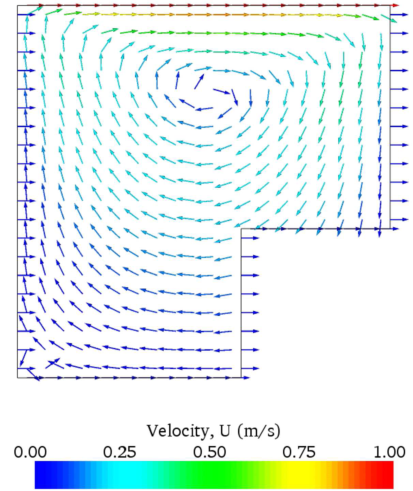
\includegraphics{fig-2-13}
 \caption{\OFcase{cavity}ケースで解いた速度場を
 \OFcase{cavityClipped}上にマッピングした図}
 \label{fig:2.13}
\end{figure}


\begin{figure}[ht]
 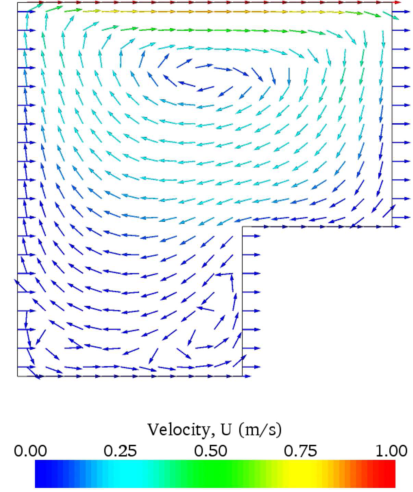
\includegraphics{fig-2-14}
 \caption{速度場の\OFcase{cavityClipped}の解法}
 \label{fig:2.14}
\end{figure}


\OFkeyword{cuttingPatches}リストは,対象パッチを削除した,
元の場の内部の値を写像した対象のパッチを含みます.
本ケースでは,\OFpatch{fixedWalls}を内挿プロセスの実例説明に用いることとします.
\begin{OFverbatim}[file]
cuttingPatches
(
  fixedWalls
);
\end{OFverbatim}
ここで,\OFtool{mapFields}を次のコマンドから実行することができます.
\begin{OFverbatim}[terminal]
mapFields ../cavity
\end{OFverbatim}
\autoref{fig:2.13}に示すような場を確認することができます.
境界パッチは,期待したように元のケースからの値が引き継がれています.
この実例において,\OFpatch{fixedWalls}パッチの速度を$(0, 0, 0)$に
リセットしたい場合があります.このときは,\OFpath{U}をエディタで開き,
\OFpatch{fixedWalls}を\OFkeyword{nonuniform}から
\OFkeyword{uniform (0,0,0)}に変更します.
そして,\OFtool{icoFoam}を実行しましょう.


\subsection{修正した形状の後処理}
\label{ssec:2.1.10}
最初と最後の解析の比較のために,この解析ケースのベクトル図を,
最初の時刻は$0.5\unit{s}$,
次いで$0.6\unit{s}$のように作成することができます.
さらに,幾何形状のアウトラインも示しますが,
これは2次元のケースでは少し注意が必要です.
\PVmenu{Filter}メニューから\PVfilter{Extract Parts}を選択し,
\PVpanel{Parameter}パネルで,興味のあるパッチ,
つまり\OFpatch{lid}と\OFpatch{fixedWalls}をハイライトします.
\PVbutton{Apply}ボタンをクリックし,\PVpanel{Display}パネルで
\PVkeyword{Wireframe}の選択すれば,
ジオメトリのうち選択したものを表示することができます.
\autoref{fig:2.14}は,パッチを黒で表示し,
修正した形状の底部角部分において形成される渦を示しています.



\section{穴あき板の応力解析}
\label{sec:2.2}
\index{あなあきいたのおうりょくかいせき@穴あき板の応力解析}%
\index{チュートリアル!あなあきいたのおうりょくかいせき@穴あき板の応力解析}%
本チュートリアルでは,中央に円形の穴を有する正方形板の
線形弾性定常応力解析における前処理,
実行および後処理の方法を述べます.
板の大きさは,辺長$4\unit{m}$および穴の半径$0.5\unit{m}$です.
さらに\autoref{fig:2.15}に示すように,
板の左右端には$\sigma = 10\unit{kPa}$の一様表面力が負荷されています.
本形状においては二つの対称面が存在するため,
解析領域は\autoref{fig:2.15}のグレーで示した板全体の
4分の1の部分のみをカバーすれば十分です.


\begin{figure}[ht]
 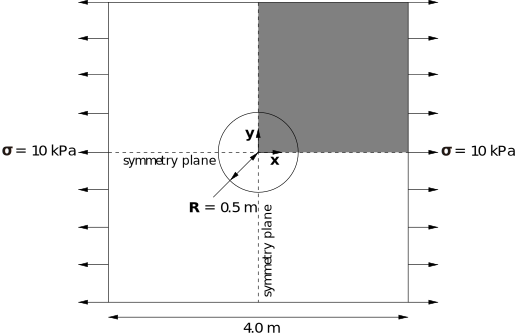
\includegraphics{fig-2-15}
 \caption{穴あき板の形状}
 \label{fig:2.15}
\end{figure}


本問題では,板の面内に応力が負荷されるため,
2次元問題として近似することができます.
デカルト座標系においては,
この構造の3番目の次元についての振る舞いを考察するにあたって,
以下の二つの仮定をすることができます.
(1) 平面応力条件:2次元平面内以外の方向にはたらく応力成分を無視できるものと仮定します.
(2) 平面ひずみ条件:2次元平面内以外の方向にはたらくひずみ成分を無視できるものと仮定します.
本ケースのように3次元方向に薄い固体に対しては,
平面応力条件が適当です.
なお平面ひずみ条件は,3次元方向に厚い固体に対して適用されます.

円形の穴を有する無限大に大きく薄い板への負荷に対しては,
解析解が存在します.垂直な対称面における法線方向応力の解は以下となります.
\begin{align}
 \label{eq:2.14}
 (\sigma_{xx})_{x=0} =
 \begin{cases}
  \displaystyle
  \sigma\left(1 + \frac{R^{2}}{2y^{2}} + \frac{3R^{4}}{2y^{4}}\right)
  & \text{for}\ |y| \ge R \\
  0 & \text{for}\ |y| < R
 \end{cases}
\end{align}
シミュレーションの実行結果をこの解析解と比較することとしましょう.
チュートリアルの最後に,
メッシュの解像度および非等間隔化に対する解の感度を調べ,
また,穴に対する板の大きさを大きくすることで
無限大板に対する解析解と有限板に対する本問題の解を比較して
誤差を見積もることができるように演習問題を用意しています.


\subsection{メッシュ生成}
\label{ssec:2.2.1}
解析領域は4ブロックからなり,
そのうちのいくつかは円弧形の端部を有します.
$x$--$y$平面におけるメッシュブロックの構造を
\autoref{fig:2.16}に示します.
\autoref{sssec:2.1.1.1}で述べたように,
2次元として扱われるようなケースであっても,
OpenFOAMでは全てのジオメトリが3次元で生成されます.
したがって$z$方向のブロックの大きさを設定しなければなりませんので,
ここでは$0.5\unit{m}$とします.
表面力境界条件は力でなく応力で指定されますので,
断面積すなわち$z$方向の大きさは解に影響を与えません.


\begin{figure}[ht]
 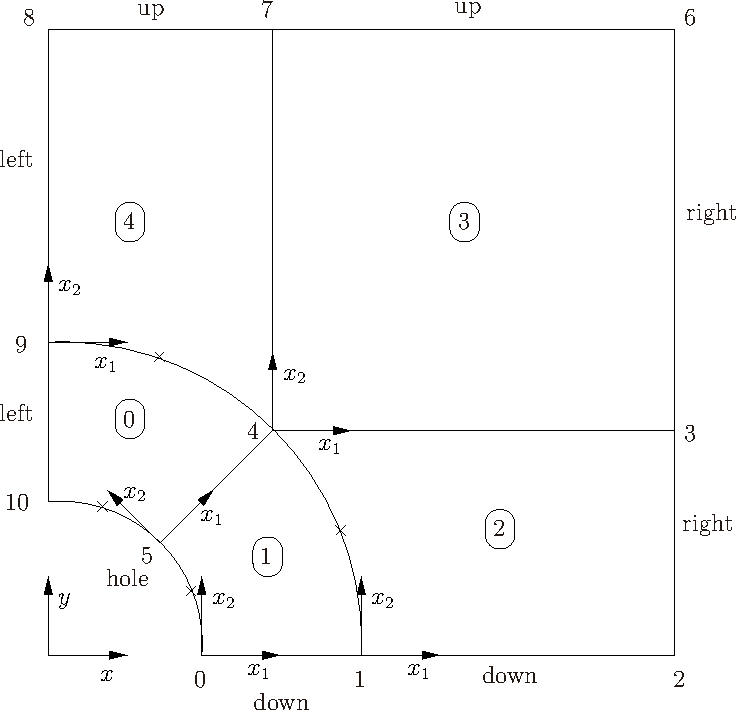
\includegraphics{fig-2-16}
 \caption{穴あき板解析のためのメッシュのブロック構造}
 \label{fig:2.16}
\end{figure}


\OFpath{\$FOAM\_RUN/tutorials/stressAnalysis/solidDisplacementFoam}ディレクトリの
\OFpath{plateHole}ケースに移動し,\OFpath{plateHole}ケースの
\OFpath{constant/polyMesh/blockMeshDict}をエディタで開きます.
\OFdictionary{block\-MeshDict}ディクショナリのエントリを以下に示します.
\begin{OFverbatim}[file, linenum=17]
convertToMeters 1;

vertices
(
    (0.5 0 0)
    (1 0 0)
    (2 0 0)
    (2 0.707107 0)
    (0.707107 0.707107 0)
    (0.353553 0.353553 0)
    (2 2 0)
    (0.707107 2 0)
    (0 2 0)
    (0 1 0)
    (0 0.5 0)
    (0.5 0 0.5)
    (1 0 0.5)
    (2 0 0.5)
    (2 0.707107 0.5)
    (0.707107 0.707107 0.5)
    (0.353553 0.353553 0.5)
    (2 2 0.5)
    (0.707107 2 0.5)
    (0 2 0.5)
    (0 1 0.5)
    (0 0.5 0.5)
);

blocks
(
    hex (5 4 9 10 16 15 20 21) (10 10 1) simpleGrading (1 1 1)
    hex (0 1 4 5 11 12 15 16) (10 10 1) simpleGrading (1 1 1)
    hex (1 2 3 4 12 13 14 15) (20 10 1) simpleGrading (1 1 1)
    hex (4 3 6 7 15 14 17 18) (20 20 1) simpleGrading (1 1 1)
    hex (9 4 7 8 20 15 18 19) (10 20 1) simpleGrading (1 1 1)
);

edges
(
    arc 0 5 (0.469846 0.17101 0)
    arc 5 10 (0.17101 0.469846 0)
    arc 1 4 (0.939693 0.34202 0)
    arc 4 9 (0.34202 0.939693 0)
    arc 11 16 (0.469846 0.17101 0.5)
    arc 16 21 (0.17101 0.469846 0.5)
    arc 12 15 (0.939693 0.34202 0.5)
    arc 15 20 (0.34202 0.939693 0.5)
);

boundary
(
    left
    {
        type symmetryPlane;
        faces
        (
            (8 9 20 19)
            (9 10 21 20)
        );
    }
    right
    {
        type patch;
        faces
        (
            (2 3 14 13)
            (3 6 17 14)
        );
    }
    down
    {
        type symmetryPlane;
        faces
        (
            (0 1 12 11)
            (1 2 13 12)
        );
    }
    up
    {
        type patch;
        faces
        (
            (7 8 19 18)
            (6 7 18 17)
        );
    }
    hole
    {
        type patch;
        faces
        (
            (10 5 16 21)
            (5 0 11 16)
        );
    }
    frontAndBack
    {
        type empty;
        faces
        (
            (10 9 4 5)
            (5 4 1 0)
            (1 4 3 2)
            (4 7 6 3)
            (4 9 8 7)
            (21 16 15 20)
            (16 11 12 15)
            (12 13 14 15)
            (15 14 17 18)
            (15 18 19 20)
        );
    }
);

mergePatchPairs
(
);

// ************************************************************************* //
\end{OFverbatim}
ここまで前のチュートリアルのように
直線的なエッジの形状を対象としてきましたが,
本チュートリアルでは曲線のエッジについて定義する必要があります.
\OFkeyword{edges}のキーワードエントリ(曲線エッジのリスト)内で
曲線エッジが定義されています.
それらのリストの構文では,最初に\OFkeyword{arc},
\OFkeyword{simpleSpline},\OFkeyword{polyLine}などの
曲線タイプが示されていますが,
さらに詳しくは\autoref{ssec:5.3.1}を参照してください.
この例題ではすべてのエッジが円弧なので\OFkeyword{arc}を使用します.
曲線を\OFkeyword{arc}で定義する際は始点と終点および
円弧上の点の3点によって指定します.

この
\index{blockMeshDict@\OFdictionary{blockMeshDict}!ディクショナリ}%
\index{ディクショナリ!blockMeshDict@\OFdictionary{blockMeshDict}}%
\OFdictionary{blockMeshDict}に含まれるブロック全てが
同じ方向を向いているわけではありません.
\autoref{fig:2.16}に示すように,
ブロック0の$x_{2}$方向はブロック4の$-x_{1}$方向と同じになっています.
このためブロック界面でセルが矛盾なく合うよう,
それぞれのブロックにおけるセルの番号および順序を
決定する際には注意を払わねばなりません.

プレートの全側面,穴の面,前後面の六つのパッチが定義されます.
そのうち左の面 (\OFpatch{left}) と下の面 (\OFpatch{down}) は対称面です.
このようなことはジオメトリ上の制限であるため,
ただの場の境界条件とするよりはメッシュの定義の中に組み込んで作ります.
よって,このパッチは\OFdictionary{blockMeshDict}内の
特別な\OFkeyword{SymmetryPlane}タイプを
使って定義するとよいでしょう.
\OFpatch{frontAndBack}パッチは2次元問題の場合は
無視される面を示しています.
これは先ほども言ったようにジオメトリ上の制限なので,
\OFdictionary{blockMeshDict}内の\OFkeyword{empty}タイプを使って定義しましょう.
境界条件に関してさらに詳しくは\autoref{ssec:5.2.1}を参照してください.
そのほかのパッチは通常の\OFkeyword{patch}タイプです.
メッシュは\OFtool{blockMesh}を使って生成し,
\autoref{ssec:2.1.2}に述べたようにして\OFtool{paraFoam}で見ることができます.
メッシュは\autoref{fig:2.17}のようになります.


\begin{figure}[ht]
 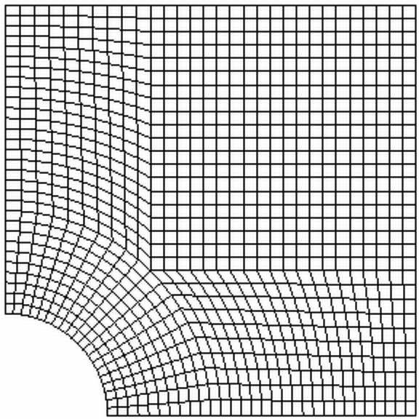
\includegraphics{fig-2-17}
 \caption{穴あき板問題のための解析メッシュ}
 \label{fig:2.17}
\end{figure}


\subsubsection{境界および初期条件}
\label{sssec:2.2.1.1}
メッシュの生成ができたら初期条件と境界条件を設定します.
熱抵抗を考慮しない応力解析では,
変位\OFkeyword{D}のみ設定する必要があります.
\OFpath{0/D}のファイルは以下のようになります.
\begin{OFverbatim}[file, linenum=17]
dimensions      [0 1 0 0 0 0 0];

internalField   uniform (0 0 0);

boundaryField
{
    left
    {
        type            symmetryPlane;
    }
    right
    {
        type            tractionDisplacement;
        traction        uniform ( 10000 0 0 );
        pressure        uniform 0;
        value           uniform (0 0 0);
    }
    down
    {
        type            symmetryPlane;
    }
    up
    {
        type            tractionDisplacement;
        traction        uniform ( 0 0 0 );
        pressure        uniform 0;
        value           uniform (0 0 0);
    }
    hole
    {
        type            tractionDisplacement;
        traction        uniform ( 0 0 0 );
        pressure        uniform 0;
        value           uniform (0 0 0);
    }
    frontAndBack
    {
        type            empty;
    }
}

// ************************************************************************* //
\end{OFverbatim}
まず,変位の初期条件が$(0, 0, 0)\unit{m}$になっています.
\OFpath{Constant/polyMesh/boundaries}のメッシュの記述にあるように,
\OFpatch{left}と\OFpatch{down}のパッチは
\OFkeyword{type}が\OFkeyword{symmetryPlane}である必要があります.
同様に\OFpatch{frontAndBack}は\OFkeyword{empty}になります.

その他のパッチは表面力境界条件です.表面力境界条件は,
(1) キーワード
\index{traction@\OFkeyword{traction}!キーワード}%
\index{キーワード!traction@\OFkeyword{traction}}%
\OFkeyword{traction}で表される,境界面における表面力ベクトル,
(2) キーワード
\index{pressure@\OFkeyword{pressure}!キーワード}%
\index{キーワード!pressure@\OFkeyword{pressure}}%
\OFkeyword{pressure}で表される,
境界面の法線方向に働く表面力となる(外向きの場合は負値となる)圧力,
の線形結合で指定されます.
\OFpatch{up}および\OFpatch{hole}パッチは表面力ゼロであるため,
表面力ベクトルおよび圧力ともにゼロが設定されます.
\OFpatch{right}パッチについては,\autoref{fig:2.24}に示すように,
表面力ベクトルは$(1\mathrm{e}4, 0, 0)\unit{Pa}$,
圧力は$0\unit{Pa}$が設定されます.
変位の初期条件は全て$(0, 0, 0)\unit{m}$が設定されます.

\subsubsection{機械的性質}
\label{sssec:2.2.1.2}
本ケースにおける物性値は
\index{mechanicalProperties@\OFdictionary{mechanicalProperties}!ディクショナリ}%
\index{ディクショナリ!mechanicalProperties@\OFdictionary{mechanicalProperties}}%
\OFdictionary{mechanicalProperties}ディクショナリによって設定します.
本問題においては,\autoref{tbl:2.1}に示す
鋼の機械的性質を指定する必要があります.
さらに本ディクショナリで\OFkeyword{planeStress}を\OFkeyword{yes}に設定しなければなりません.


\begin{table}[ht]
 %#! platex UserGuideJa
\begin{tabular}{lccc}
 物性 & 単位 & キーワード & 値 \\
 \hline
 密度 & $\unit*{kg\,m^{-3}}$ & \OFkeyword{rho} & 7854 \\
 ヤング率 & $\unit*{Pa}$ & \OFkeyword{E} & $2 \times 10^{11}$ \\
 ポアソン比 & --- & \OFkeyword{nu} & 0.3 \\
 \hline
\end{tabular}

 \caption{鋼の機械的性質}
 \label{tbl:2.1}
\end{table}


\subsubsection{熱的性質}
\label{sssec:2.2.1.3}
運動によって発生する熱応力によって
運動方程式と連成した熱方程式を解くことができるよう,
\index{solidDisplacementFoam@\OFtool{solidDisplacementFoam}!ソルバ}%
\index{ソルバ!solidDisplacementFoam@\OFtool{solidDisplacementFoam}}%
\OFtool{solidDisplacementFoam}ソルバには温度場を表す変数\OFkeyword{T}が存在します.
\index{thermalProperties@\OFdictionary{thermalProperties}!ディクショナリ}%
\index{ディクショナリ!thermalProperties@\OFdictionary{thermalProperties}}%
\OFdictionary{thermalProperties}ディクショナリの\OFkeyword{thermalStress}スイッチによって,
OpenFOAMが熱方程式を解くべきかどうかを実行時に指定します.
また本ディクショナリによって,
本ケースすなわち\autoref{tbl:2.2}に示す
鋼の熱的性質を指定します.


\begin{table}[ht]
 %#! platex ProgrammersGuideJa
\begin{tabular}{|cccc|}
 \hline
 \tblstrut
 項の記述 & 陰的・陽的 & 記述 & \OFclass{fvm::}または\OFclass{fvc::}の関数 \\
 \hline\hline
 \tblstrut
 ラプラシアン & 陰的・陽的 & $\nabla^{2}\phi$ & \texttt{laplacian(phi)} \\
 &  & $\nabla \inProd \varGamma \nabla \phi$ & \texttt{laplacian(Gamma, phi)} \\
 \hline
 \tblstrut
 時間微分 & 陰的・陽的 & $\frac{\partial\phi}{\partial t}$ & \texttt{ddt(phi)} \\
 &  & $\frac{\partial\rho\phi}{\partial t}$ & \texttt{ddt(rho, phi)} \\
 \hline
 \tblstrut
 時間の2階微分 & 陰的・陽的 & $\frac{\partial}{\partial t}\left(\rho\frac{\partial\phi}{\partial t}\right)$ & \texttt{d2dt2(rho, phi)} \\
 \hline
 \tblstrut
 移流 & 陰的・陽的 & $\nabla \inProd (\psi)$ & \verb|div(psi, scheme)*| \\
 &  & $\nabla \inProd (\psi\phi)$ & \verb|div(psi, phi, word)*| \\
 &  &  & \verb|div(psi, phi)| \\
 \hline
 \tblstrut
 発散 & 陽的 & $\nabla \inProd \chi$ & \texttt{div(chi)} \\
 \hline
 \tblstrut
 勾配 & 陽的 & $\nabla \chi$ & \texttt{grad(chi)} \\
 &  & $\nabla \phi$ & \texttt{gGrad(phi)} \\
 &  &  & \texttt{lsGrad(phi)} \\
 &  &  & \texttt{snGrad(phi)} \\
 &  &  & \texttt{snGradCorrection(phi)} \\
 \hline
 \tblstrut
 勾配の勾配の二乗 & 陽的 & $|\nabla\nabla\phi|^{2}$ & \texttt{sqrGradGrad(phi)} \\
 \hline
 \tblstrut
 回転 & 陽的 & $\nabla \times \phi$ & \texttt{curl(phi)} \\
 \hline
 \tblstrut
 湧き出し & 陰的 & $\rho\phi$ & \texttt{Sp(rho, phi)} \\
 & 陰的・陽的\textsuperscript{\dag} &  & \texttt{SuSp(rho, phi)} \\
 \hline
 \multicolumn{4}{l}{\tblstrut\dag\ 湧き出し\OFkeyword{fvm::SuSp}は
 \OFkeyword{rho}の符号に依存して,陰的または陽的に離散化されます.} \\
 \multicolumn{4}{l}{\dag\ 陽的な湧き出しは単純に
 \OFclass{vol<Type>Field}で指定されます.例:\texttt{rho*phi}} \\
 \multicolumn{4}{l}{関数の引数は以下のようなクラスです.} \\
 \multicolumn{4}{l}{\OFkeyword{phi}: \OFclass{vol<Type>Field}} \\
 \multicolumn{4}{l}{\OFkeyword{Gamma}: \OFclass{scalar},\OFclass{volScalarField},
 \OFclass{volTensorField},\OFclass{surfaceTensorField}.} \\
 \multicolumn{4}{l}{\OFkeyword{rho}: \OFclass{scalar},\OFclass{volScalarField}} \\
 \multicolumn{4}{l}{\OFkeyword{psi}: \OFclass{surfaceTensorField}} \\
 \multicolumn{4}{l}{\OFkeyword{chi}: \OFclass{surface<Type>Field},\OFclass{vol<Type>Field}} \\
\end{tabular}

 \caption{鋼の熱的性質}
 \label{tbl:2.2}
\end{table}


本ケースにおいては熱の方程式は解きません.
したがって\OFdictionary{thermalProperties}ディクショナリにおける
\OFkeyword{thermalStress}キーワードエントリは\OFkeyword{no}に設定します.

\subsubsection{制御}
\label{sssec:2.2.1.4}
通常どおり,解法の制御に関する情報は\OFdictionary{controlDict}ディクショナリから
読み込まれます.本ケースでは,\OFkeyword{startTime}は0です.
本ケースは定常状態ですので,時間刻みは重要ではありません.
このような状況では,
定常状態のケースにおける反復回数カウンタとして働くよう,
時間刻み\OFkeyword{deltaT}を1に設定するのが最善です.
このようにした場合,本ケースで100に設定した\OFkeyword{endTime}は
反復回数の上限として働きます.\OFkeyword{writeInterval}は20に設定します.

\index{controlDict@\OFdictionary{controlDict}!ディクショナリ}%
\index{ディクショナリ!controlDict@\OFdictionary{controlDict}}%
\OFdictionary{controlDict}のエントリは以下のようになります.
\begin{OFverbatim}[file, linenum=17]

application     solidDisplacementFoam;

startFrom       startTime;

startTime       0;

stopAt          endTime;

endTime         100;

deltaT          1;

writeControl    timeStep;

writeInterval   20;

purgeWrite      0;

writeFormat     ascii;

writePrecision  6;

writeCompression off;

timeFormat      general;

timePrecision   6;

graphFormat     raw;

runTimeModifiable true;


// ************************************************************************* //
\end{OFverbatim}

\subsubsection{離散化スキームおよび線形方程式ソルバ制御}
\label{sssec:2.2.1.5}
次は\OFdictionary{fvSchemes}ディクショナリについて見てみましょう.
まず,この問題は定常状態ですので,
\OFkeyword{timeScheme}における時間微分としては\OFkeyword{steadyState}を選択します.
これによって時間微分項がオフの状態になります.
全てのソルバが定常状態および過渡的状態の双方に対して
適用可能な訳ではありませんが,
\OFtool{solidDisplacementFoam}は基本的なアルゴリズムが
双方のシミュレーションともに共通であるため,
双方に適用可能となっています.

線形弾性応力解析における運動方程式には,
変位の勾配を含む陽な項がいくつか存在します.
この勾配を正確かつ滑らかに評価できれば,良い計算結果が得られます.
通常,有限体積法における離散化は,
\index{こうばい@勾配!ガウスのていり@ガウスの定理}%
ガウスの定理に基づいています.
ガウス法は大抵の目的においては十分に正確ですが,
本ケースにおいては
\index{こうばい@勾配!さいしょうじじょうフィット@最小二乗フィット}%
\index{こうばい@勾配!さいしょうじじょうほう@最小二乗法}%
最小二乗法を使用することとします.
したがって
\index{fvSchemes@\OFdictionary{fvSchemes}!ディクショナリ}%
\index{ディクショナリ!fvSchemes@\OFdictionary{fvSchemes}}%
\OFdictionary{fvSchemes}ディクショナリを開き,
\OFkeyword{grad(U)}勾配離散化スキームとして
\index{leastSquares@\OFkeyword{leastSquares}!キーワード}%
\index{キーワード!leastSquares@\OFkeyword{leastSquares}}%
\OFkeyword{leastSquares}を選択してください.
\begin{OFverbatim}[file, linenum=17]

d2dt2Schemes
{
    default         steadyState;
}

gradSchemes
{
    default         leastSquares;
    grad(D)         leastSquares;
    grad(T)         leastSquares;
}

divSchemes
{
    default         none;
    div(sigmaD)     Gauss linear;
}

laplacianSchemes
{
    default         none;
    laplacian(DD,D) Gauss linear corrected;
    laplacian(DT,T) Gauss linear corrected;
}

interpolationSchemes
{
    default         linear;
}

snGradSchemes
{
    default         none;
}

fluxRequired
{
    default         no;
    D               yes;
    T               no;
}


// ************************************************************************* //
\end{OFverbatim}
\OFpath{system}ディレクトリにある
\OFdictionary{fvSolution}ディクショナリでは,
求解に使用される線形方程式のソルバおよびアルゴリズムを設定します.
まず\OFsubdictionary{solvers}サブディクショナリを見ると,
\OFkeyword{D}の
\index{solver@\OFkeyword{solver}!キーワード}%
\index{キーワード!solver@\OFkeyword{solver}}%
\OFkeyword{solver}が
\index{GAMG@\OFkeyword{GAMG}!キーワードエントリ}%
\index{キーワードエントリ!GAMG@\OFkeyword{GAMG}}%
\OFkeyword{GAMG}になっていることがわかります.
\index{tolerance@\OFkeyword{tolerance}!キーワード}%
\index{キーワード!tolerance@\OFkeyword{tolerance}}%
\OFkeyword{tolerance}で表される
ソルバ許容値(ソルバ名の次の数値)は,本問題では$10^{-6}$を設定します.
\index{relTol@\OFkeyword{relTol}!キーワード}%
\index{キーワード!relTol@\OFkeyword{relTol}}%
\OFkeyword{relTol}で表される
ソルバの相対許容値(さらにその次の数値)には
各反復ごとの残差の所要低減量を設定します.
本問題においては多くの項が陽であり,
また個別の反復的手順の一部としてアップデートされるため,
各反復において厳しい相対許容値を設定することは非効率的です.
したがって相対許容値として合理的な値は$0.01$,
もしくはさらに高めの$0.1$,
あるいはせいぜいこのケースのように$0.9$程度にしておきます.
\begin{OFverbatim}[file, linenum=17]

solvers
{
    "(D|T)"
    {
        solver          GAMG;
        tolerance       1e-06;
        relTol          0.9;
        smoother        GaussSeidel;
        cacheAgglomeration true;
        nCellsInCoarsestLevel 20;
        agglomerator    faceAreaPair;
        mergeLevels     1;
    }
}

stressAnalysis
{
    compactNormalStress yes;
    nCorrectors     1;
    D               1e-06;
}


// ************************************************************************* //
\end{OFverbatim}
\OFdictionary{fvSolution}ディクショナリは,
アプリケーションソルバに特有の制御パラメータを含む
\OFsubdictionary{stressAnalysis}サブディクショナリを含みます.
まず,各時刻ステップ内での表面力境界条件処理を含めた,
全方程式系に関する外側ループの数を指定する\OFkeyword{nCorrectors}があります.
本問題は定常状態を扱いますので,
「時刻ステップ」を反復回数カウンタとして使い収束解へと向かう
反復を実行することになります.
したがって\OFkeyword{nCorrectors}を1に設定します.

\OFkeyword{D}キーワードには外側反復ループにおける収束許容値,
すなわち初期残差に対して反復計算によって消去されるべき
レベルを設定します.
本問題では前述において設定したソルバ許容値の$10^{-6}$に設定します.


\subsection{コードの実行}
\label{ssec:2.2.2}
以下に示すようなコマンドによって,
実行後にログファイルに記録された収束状況を見ることができるよう,
バックグラウンドでコードを実行します.
\begin{OFverbatim}[terminal]
cd $FOAM_RUN/tutorials/stressAnalysis/solidDisplacementFoam/plateHole
solidDisplacementFoam > log &
\end{OFverbatim}%$
実行後には生成されたログファイルを見て,
反復回数および解を求める各方向変位の初期・最終残差などの
収束状況を確認できます.
本ケースの反復許容回数設定では,
最終残差は必ず初期残差の$0.1$倍以下となるはずです.
いったん両初期残差ともに$10^{-6}$の収束許容残差以下となれば,
その計算は収束したとみなしバッチジョブを\texttt{kill}することによって
止めることができます.


\subsection{後処理}
\label{ssec:2.2.3}
後処理は\autoref{ssec:2.1.4}と
同様に行うことができます.
\OFtool{solidDisplacementFoam}ソルバは,
応力場$\sigma$を対称テンソル場として出力します.
したがって例えば,$\sigma_{xx}$を\OFtool{paraFoam}で見ることができます.
OpenFOAMソルバにおける変数名は通常,
それらを表す数学記号にならって名付けられることは,
ここで再度述べるに値するでしょう.ギリシア記号の場合は,
変数は発音どおりに名付けられます.例えば,
$\sigma_{xx}$は\OFkeyword{sigmaxx}と名付けられます.

独立したスカラ成分の$\sigma_{xx}$や$\sigma_{xy}$などは,
\autoref{sssec:2.1.5.7}で述べた\OFtool{foamCalc}を\OFkeyword{sigma}に関して実行して求めます.
\begin{OFverbatim}[terminal]
foamCalc components sigma
\end{OFverbatim}
\OFkeyword{sigmaxx}や\OFkeyword{sigmaxy}などと名づけられた成分の
ファイルが時間のディレクトリに生成されます.
\autoref{fig:2.18}のように応力を\OFtool{paraFoam}で見ることができます.


\begin{figure}[ht]
 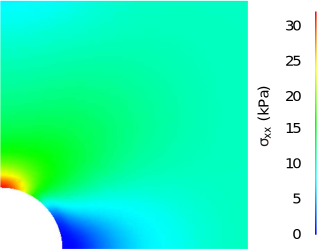
\includegraphics{fig-2-18}
 \caption{穴あき板における応力場}
 \label{fig:2.18}
\end{figure}


\autoref{eq:2.14} の解析解と
ここで得られた数値解を比較しましょう.
そのためには,解析領域左端の対称面に沿ってのデータを
出力しなければなりません.
このようなグラフのために必要なデータは,
\OFtool{sample}ユーティリティによって作成することができます.
\OFtool{sample}の設定は\OFpath{system}ディレクトリ内の\OFpath{sampleDict}で行い
詳細は\autoref{tbl:6.3}に要約しています.
データのサンプリングを行う座標区間は,
\OFkeyword{sets}によって$(0.0, 0.5, 0.25)$から$(0.0, 2.0, 0.25)$に指定されています.
物理量は\OFkeyword{fields}に指定します.
\begin{OFverbatim}[file, linenum=17]

interpolationScheme cellPoint;

setFormat       raw;

sets
(
    leftPatch
    {
        type    uniform;
        axis    y;
        start   ( 0 0.5 0.25 );
        end     ( 0 2 0.25 );
        nPoints 100;
    }
);

fields          ( sigmaxx );


// ************************************************************************* //
\end{OFverbatim}
通常通り\OFtool{sample}を実行してください.
\index{writeFormat@\OFkeyword{writeFormat}!キーワード}%
\index{キーワード!writeFormat@\OFkeyword{writeFormat}}%
\OFkeyword{writeFormat}は\OFkeyword{raw}形式で2列のフォーマットとなっています.
データは\OFpath{sets}ディレクトリの時刻サブディレクトリの中のファイルに書き込まれます.
たとえば,時刻$t = 100\unit{s}$のデータは
\OFpath{sets/100/leftPatch\_sigmaxx.xy}に書き込まれます.
GnuPlotのようなアプリケーションでは,
コマンドプロンプトで以下を入力することで,
数値解および解析解の両方をプロットすることができます.
\begin{OFverbatim}[terminal]
plot [0.5:2] [0:] 'sets/100/leftPatch_sigmaxx.xy',
     1e4*(1+(0.125/(x**2))+(0.09375/(x**4)))
\end{OFverbatim}
プロット例を\autoref{fig:2.19}に示します.


\begin{figure}[ht]
 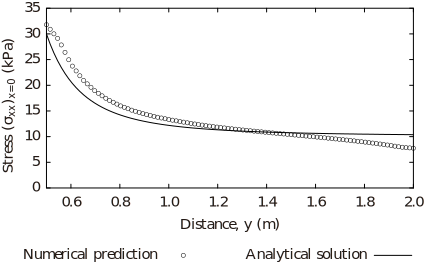
\includegraphics{fig-2-19}
 \caption{垂直方向対称面における法線方向応力}
 \label{fig:2.19}
\end{figure}


\subsection{演習}
\label{ssec:2.2.4}
以下は\OFtool{solidDisplacementFoam}に習熟していただくための演習課題です.

\subsubsection{メッシュ解像度の増加}
\label{sssec:2.2.4.1}
$x$,$y$方向それぞれのメッシュ解像度を増やしてみましょう.
\autoref{ssec:2.2.3}の最終的な粗メッシュの結果を,
\index{mapFields@\OFtool{mapFields}!ユーティリティ}%
\index{ユーティリティ!mapFields@\OFtool{mapFields}}%
\OFtool{mapFields}を使って密メッシュの初期条件にマッピングしてください.

\subsubsection{非等間隔メッシュの導入}
\label{sssec:2.2.4.2}
穴に近いセルが遠いセルより密になるよう,
メッシュ幅を変化させてください.
隣接するセルの大きさの比率が$1.1$以上にならないように,
またブロック間のセルの大きさの比率がブロック内の比率と
同様となるようメッシュを作成してください.
メッシュの非等間隔化については\autoref{ssec:2.1.6}で述べました.
ここでも,\autoref{ssec:2.2.3}の最終的な粗メッシュでの結果を,
\OFtool{mapFields}を使って非等間隔メッシュの初期条件としてマッピングします.
結果を解析解および非等間隔化する前の結果と比較してみましょう.
等間隔メッシュと同一のセル数を使用した場合,
解の精度は改善されるでしょうか?

\subsubsection{板の大きさの変更}
\label{sssec:2.2.4.3}
ここで示されている解析解は,
有限な大きさの穴を有する無限大板におけるものです.
したがって有限な大きさの板においては,
この解析解は必ずしも正確ではありません.
誤差を見積もるために,
穴の大きさを同一に保ったまま板を大きくしてみましょう.



\section{ダムの決壊}
\label{sec:2.3}
\index{ダムのけっかい@ダムの決壊}%
\index{チュートリアル!ダムのけっかい@ダムの決壊}%
このチュートリアルでは,\OFtool{interFoam}を用いて,
単純化したダム決壊の2次元問題を解くことにします.
この問題の特徴は,くっきりとした界面や
\index{じゆうひょうめん@自由表面}%
自由表面によって
隔てられている二つの流体による非定常の流れ場であることです.
\OFtool{interFoam}における2相流体を解くアルゴリズムは,
Volume of fluid (VOF) 法によるものであり,
ここでは特別な輸送方程式を解いて,
計算格子における2相の体積分率,
もしくは相比率$\alpha_{1}$を決定します.
各物理量は,この相比率に(各流体の)密度をかけた
平均的な値として算出されます.
個々の物質の界面は,VOF法ではその性質上明示的には解かれず,
相比率場の特性として浮き上がってくるということになります.
相比率は0から1の間の任意の値をとり得るため,
界面は決してくっきりと定義されませんので,
本来のくっきりとした界面が存在するべき領域の周辺を,
(計算上の)界面がぼんやりと占めることになります.

計算条件では,貯水池の左側に,膜で仕切られた水柱が最初存在します.
時刻$t = 0\unit{s}$に,膜が取り除かれて,水柱が崩れだします.
崩壊しながら,水流は貯水槽の底にある出っ張りにぶつかり,
いくつかの気泡を含む,複雑な流れ場の様相を呈します.
計算形状と初期条件は\autoref{fig:2.20}に示しました.


\begin{figure}[ht]
 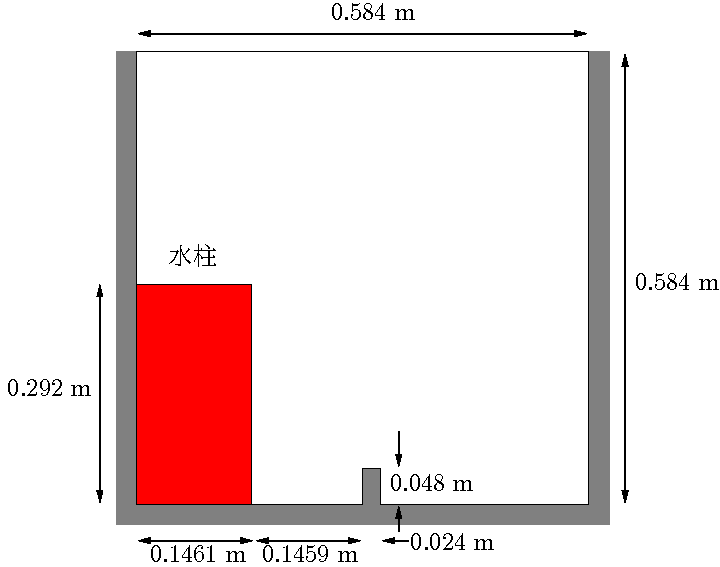
\includegraphics{fig-2-20}
 \caption{ダム決壊の計算形状}
 \label{fig:2.20}
\end{figure}


\subsection{格子の生成}
\label{ssec:2.3.1}
\OFpath{\$FOAM\_RUN/tutorials/multiphase/interFoam/laminar}にある
\OFpath{damBreak}のケースディレクトリに移動しましょう.
前述した方法で\OFtool{blockMesh}を実行して格子を生成してください.
この\OFcase{damBreak}のメッシュは五つのブロックで構成されます.
\OFdictionary{blockMeshDict}の中身を以下に示します.
\begin{OFverbatim}[file, linenum=17]

convertToMeters 0.146;

vertices        
(
    (0 0 0)
    (2 0 0)
    (2.16438 0 0)
    (4 0 0)
    (0 0.32876 0)
    (2 0.32876 0)
    (2.16438 0.32876 0)
    (4 0.32876 0)
    (0 4 0)
    (2 4 0)
    (2.16438 4 0)
    (4 4 0)
    (0 0 0.1)
    (2 0 0.1)
    (2.16438 0 0.1)
    (4 0 0.1)
    (0 0.32876 0.1)
    (2 0.32876 0.1)
    (2.16438 0.32876 0.1)
    (4 0.32876 0.1)
    (0 4 0.1)
    (2 4 0.1)
    (2.16438 4 0.1)
    (4 4 0.1)
);

blocks          
(
    hex (0 1 5 4 12 13 17 16) (23 8 1) simpleGrading (1 1 1)
    hex (2 3 7 6 14 15 19 18) (19 8 1) simpleGrading (1 1 1)
    hex (4 5 9 8 16 17 21 20) (23 42 1) simpleGrading (1 1 1)
    hex (5 6 10 9 17 18 22 21) (4 42 1) simpleGrading (1 1 1)
    hex (6 7 11 10 18 19 23 22) (19 42 1) simpleGrading (1 1 1)
);

edges           
(
);

boundary
(
    leftWall
    {
        type wall;
        faces
        (
            (0 12 16 4)
            (4 16 20 8)
        );
    }
    rightWall
    {
        type wall;
        faces
        (
            (7 19 15 3)
            (11 23 19 7)
        );
    }
    lowerWall
    {
        type wall;
        faces
        (
            (0 1 13 12)
            (1 5 17 13)
            (5 6 18 17)
            (2 14 18 6)
            (2 3 15 14)
        );
    }
    atmosphere
    {
        type patch;
        faces
        (
            (8 20 21 9)
            (9 21 22 10)
            (10 22 23 11)
        );
    }
);

mergePatchPairs
(
);

// ************************************************************************* //
\end{OFverbatim}


\subsection{境界条件}
\label{ssec:2.3.2}
\OFpath{constant/polyMesh}ディレクトリの\OFpath{boundary}ファイルを見ることで
\OFtool{blockMesh}で生成された境界の形状を確認しましょう.
\OFpatch{leftWall},\OFpatch{rightWall},\OFpatch{lowerWall},
\OFpatch{atmosphere},\OFpatch{defaultFaces}の
五つの境界パッチがあります.
パッチの種類について理解しておきましょう.
\OFpatch{atmosphere}は何の属性もなく,
単に境界条件によって規定される標準の\OFboundary{patch}です.
\OFpatch{defaultFaces}は,本ケースでは2次元であるため
パッチの法線方向を解析の対象としないため,\OFboundary{empty}とします.
\OFpatch{leftWall},\OFpatch{rightWall},
\OFpatch{lowerWall}はそれぞれ
\index{wall@\OFboundary{wall}!きょうかいじょうけん@境界条件}%
\index{きょうかいじょうけん@境界条件!wall@\OFboundary{wall}}%
\OFboundary{wall}です.
ただの\OFboundary{patch}と同様に\OFboundary{wall}もメッシュについて形状や位相の情報をもちませんが,
壁として識別することができるので,
アプリケーションに特殊な壁表面のモデリングを明示するために
\OFboundary{wall}と定義しています.

\OFtool{interFoam}のソルバが,界面と壁面との接点における
表面張力に対するモデルを含んでいる,というのがよい例です.
このモデルは\OFkeyword{alpha1} ($\alpha_{1}$) 場の
\index{alphaContactAngle@\OFboundary{alphaContactAngle}!きょうかいじょうけん@境界条件}%
\index{きょうかいじょうけん@境界条件!alphaContactAngle@\OFboundary{alphaContactAngle}}%
\OFboundary{alphaContactAngle}の境界条件と関連付けられています.
その場合,静的な接触角度\OFkeyword{theta0} $\theta_{0}$や,
前縁や後縁における動的な接触角度である
\OFkeyword{thetaA} $\theta_{\mathrm{A}}$と\OFkeyword{thetaR} $\theta_{\mathrm{R}}$,
そして,動的な接触角度において速度に比例する係数
\OFkeyword{uTheta}を指定する必要があります.

このチュートリアルでは,壁面と界面間の表面張力による効果を
無視することにしたいと思います.
それは,静的な接触角度を$\theta_{0} = 90\degree$に,
速度比例係数を$0$と設定することで可能です.
しかしながら,壁の境界条件として,
通常の\OFkeyword{wall}タイプの境界条件を指定する別なやり方もあります.
この場合,\OFkeyword{alpha1}に対して\OFkeyword{alphaContactAngle}の境界条件を設定する代わりに,
\OFkeyword{zeroGradient}に設定します.

\OFpatch{top}の境界は大気に対して開放されていることから,
内部流れに応じて流出・流入のいずれも可能にしておく必要があります.
したがって,以下のような,安定性を維持しながらこれを可能にするような
圧力と速度に対する境界条件の組み合わせを用いることになります.
\begin{itemize}
 \item \OFboundary{totalPressure}は,与えられた全圧\OFkeyword{p0}と
       局所速度\OFkeyword{U}から計算される\OFboundary{fixedValue}条件です.
 \item \OFboundary{pressureInletOutletVelocity}は
       全成分に\OFboundary{zeroGradient}を適用しますが,
       流入がある場合は例外として\OFboundary{fixedValue}が
\OFrevision{法線成分では?}%
       \OFemph{接線}成分に適用されます
 \item \OFboundary{inletOutlet}は,流れが外向きならば\OFboundary{zeroGradient}であり,
       流れが内向きならば\OFboundary{fixedValue}です
\end{itemize}
すべての壁の境界においては,圧力場には\OFboundary{buoyantPressure}境界条件を適用しますが,
これは局所的な密度勾配から法線方向勾配を計算します.

2次元問題における前後の面を表している\OFpatch{defaultFaces}パッチは,
通常通り\OFkeyword{empty}タイプにします.


\subsection{初期条件の設定}
\label{ssec:2.3.3}
これまでのケースと異なり,ここでは相比率$\alpha_{1}$に対して,
以下のような非一様な初期条件を与えます.
\begin{align}
 \label{eq:2.15}
 \alpha_{1} =
 \begin{cases}
  1 & \text{液相} \\
  0 & \text{気相}
 \end{cases}
\end{align}
これは,
\index{setFields@\OFtool{setFields}!ユーティリティ}%
\index{ユーティリティ!setFields@\OFtool{setFields}}%
\OFtool{setFields}ユーティリティを実行することによって行います.
この実行には\OFpath{system}ディレクトリ内の\OFpath{setFieldsDict}を必要とします.
このケースにおける\OFpath{setFieldsDict}ファイルの内容を以下に示します.
\begin{OFverbatim}[file, linenum=17]

defaultFieldValues
(
    volScalarFieldValue alpha1 0
);

regions
(
    boxToCell
    {
        box (0 0 -1) (0.1461 0.292 1);
        fieldValues
        (
            volScalarFieldValue alpha1 1
        );
    }
);


// ************************************************************************* //
\end{OFverbatim}
ここで,
\index{defaultFieldValues@\OFkeyword{defaultFieldValues}!キーワード}%
\index{キーワード!defaultFieldValues@\OFkeyword{defaultFieldValues}}%
\OFkeyword{defaultFieldValues}は場の規定値を設定するものであり,
\index{regions@\OFsubdictionary{regions}!キーワード}%
\index{キーワード!regions@\OFsubdictionary{regions}}%
\OFsubdictionary{regions}のサブディクショナリにおいて別途指定されない場合に場に与えられる値です.
\OFsubdictionary{regions}のサブディクショナリは,指定された領域において,
規定値を上書きする
\index{fieldValues@\OFkeyword{fieldValues}!キーワード}%
\index{キーワード!fieldValues@\OFkeyword{fieldValues}}%
\OFkeyword{fieldValues}を含んだサブディクショナリのリストを含んでいます.
領域の定義は,ある位相幾何学的な制約に基づいて,
点や格子,界面等の集合を生成する
\index{topoSetSource@\OFkeyword{topoSetSource}!キーワード}%
\index{キーワード!topoSetSource@\OFkeyword{topoSetSource}}%
\OFkeyword{topoSetSource}によって行います.
ここでは,
\index{boxToCell@\OFkeyword{boxToCell}!キーワード}%
\index{キーワード!boxToCell@\OFkeyword{boxToCell}}%
\OFkeyword{boxToCell}を使って,大きいほうと小さいほうの
二つの座標点で定義されるバウンディング・ボックスを生成し,
液体の領域となるセルの集合を定義しています.
また,この領域における相比率$\alpha_{1}$を$1$と指定しています.

\index{setFields@\OFtool{setFields}!ユーティリティ}%
\index{ユーティリティ!setFields@\OFtool{setFields}}%
\OFtool{setFields}ユーティリティはファイルから場を読み込み,
再計算したうえで,再びファイルに書き込みます.
そのファイルは上書きされてしまうので,
\OFtool{setFields}を実行する前にバックアップをとることをお勧めします.
この\OFcase{damBreak}チュートリアルには,
\OFkeyword{alpha1}場は最初は\OFkeyword{alpha1.org}という名前の
バックアップしか置いてありません.\OFtool{setFields}を実行する前に,
まず以下のようにタイプして\OFkeyword{alpha1.org}を\OFkeyword{alpha1}にコピーする必要があります.
\begin{OFverbatim}[terminal]
cp 0/alpha1.org 0/alpha1
\end{OFverbatim}

さて,それでは
\index{setFields@\OFtool{setFields}!ユーティリティ}%
\index{ユーティリティ!setFields@\OFtool{setFields}}%
\OFtool{setFields}を他のプログラムと同様に起動してください.
そうしたら,\OFtool{paraFoam}を用いて,初期の\OFkeyword{alpha1}場が
\autoref{fig:2.21}のように望むような分布に
なっているかどうか確かめてください.


\begin{figure}[ht]
 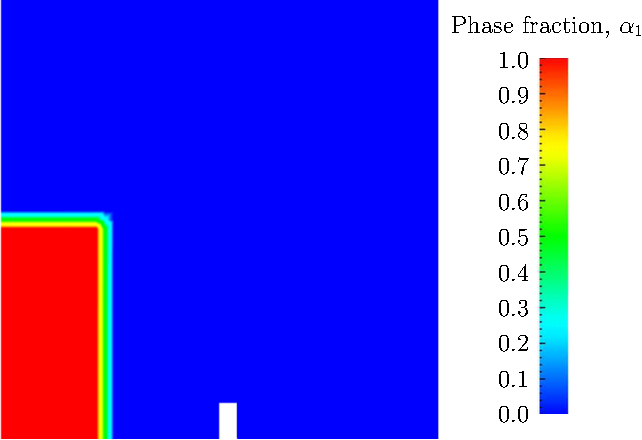
\includegraphics{fig-2-21}
 \caption{相比率\OFkeyword{alpha1}の初期条件}
 \label{fig:2.21}
\end{figure}


\subsection{流体の物性値}
\label{ssec:2.3.4}
\OFpath{constant}ディレクトリの
\index{transportProperties@\OFpath{transportProperties}!ファイル}%
\index{ファイル!transportProperties@\OFpath{transportProperties}}%
\OFpath{transportProperties}ファイルを確認しましょう.
このディクショナリは各流体の物性値を含んでおり,
二つのサブディクショナリ\OFsubdictionary{phase1}と
\OFsubdictionary{phase2}に分かれています.
各相の輸送モデルは,\OFkeyword{transportModel}によって選択されます.
ここで,動粘性係数が\OFkeyword{nu}というキーワードで指定され,
一定値である
\index{Newtonian@\OFkeyword{Newtonian}!キーワードエントリ}%
\index{キーワードエントリ!Newtonian@\OFkeyword{Newtonian}}%
\OFkeyword{Newtonian}モデルを選んでください.

\index{CrossPowerLaw@\OFkeyword{CrossPowerLaw}!キーワードエントリ}%
\index{キーワードエントリ!CrossPowerLaw@\OFkeyword{CrossPowerLaw}}%
\OFkeyword{CrossPowerLaw}といったその他のモデルにおける粘性係数の指定は,
この例における\OFsubdictionary{CrossPowerLawCoeffs}といったように,
\OFsubdictionary{<model>Coeffs}という名のサブディクショナリの中で行います.

密度の指定は,\OFkeyword{rho}キーワードで行います.

二つの相の間の表面張力は,\OFkeyword{sigma}キーワードで指定します.

このチュートリアルで用いた値を\autoref{tbl:2.3}に挙げます.


\begin{table}
 %#! platex UserGuideJa
\begin{tabular}{lccc}
 \OFkeyword{phase1}の物性 \\
 \hline
 動粘性率 & $\unit*{m^{2}s^{-1}}$ & \OFkeyword{nu} & $1.0 \times 10^{6}$ \\
 密度 & $\unit*{kg\,m^{-3}}$ & \OFkeyword{rho} & $1.0 \times 10^{3}$ \\
 \\
 \OFkeyword{phase2}の物性 \\
 \hline
 動粘性率 & $\unit*{m^{2}s^{-1}}$ & \OFkeyword{nu} & $1.48 \times 10^{-5}$ \\
 密度 & $\unit*{kg\,m^{-3}}$ & \OFkeyword{rho} & $1.0$ \\
 \\
 両相の物性 \\
 \hline
 表面張力 & $\unit*{N\,m^{^1}}$ & \OFkeyword{sigma} & $0.07$ \\
 \hline
\end{tabular}

 \caption{\OFcase{damBreak}チュートリアルにおける流体物性}
 \label{tbl:2.3}
\end{table}


重力加速度は全領域にわたって一様で,
\OFpath{constant}ディレクトリの
\index{g@\OFpath{g}!ファイル}%
\index{ファイル!g@\OFpath{g}}%
\OFpath{g}ファイルで指定されます.
\OFpath{U}や\OFpath{p}のような通常のフィールドのファイルと異なり,
\OFpath{g}は\OFclass{uniformDimensionedVectorField}であり,
単に\OFkeyword{dimensions}と\OFkeyword{value}の組だけを含みます.
このチュートリアルでは$(0, 9.81, 0)\unit{m\,s^{-2}}$です.
\begin{OFverbatim}[file, linenum=17]

dimensions      [0 1 -2 0 0 0 0];
value           ( 0 -9.81 0 );


// ************************************************************************* //
\end{OFverbatim}


\subsection{乱流モデル}
\label{ssec:2.3.5@1.6}
キャビティの例題のように,
\index{turbulenceProperties@\OFdictionary{turbulenceProperties}!ディクショナリ}%
\index{ディクショナリ!turbulenceProperties@\OFdictionary{turbulenceProperties}}%
\OFdictionary{turbulenceProperties}ディクショナリの
\index{simulationType@\OFkeyword{simulationType}!キーワード}%
\index{キーワード!simulationType@\OFkeyword{simulationType}}%
\OFkeyword{simulationType}キーワードで乱流のモデリング手法を選択することができます.
この例題は乱流モデルを使わずに実行したいので\OFkeyword{laminar}と指定します.
\begin{OFverbatim}[file, linenum=17]

simulationType  laminar;


// ************************************************************************* //
\end{OFverbatim}


\subsection{時間ステップの制御}
\label{ssec:2.3.5}
自由界面の捕捉においては,時間ステップの制御は重要です.
というのも,界面捕捉のアルゴリズムは,通常の流体計算に比べ,
クーラン数$\nCo$に対してかなり鋭敏だからです.
理想的には,界面がある領域において,
上限値として$\nCo \approx 0.5$を超えないようにすべきです.
伝播速度の予測が容易であるようなケースでは,$\nCo$の制限を守るような
固定した時間ステップを指定することができますが,
より複雑なケースの場合時間ステップの指定はずっと困難になります.
そこで,\OFtool{interFoam}では,\OFdictionary{controlDict}において,
時間ステップの自動修正を指定することをお勧めします.
\index{adjustTimeStep@\OFkeyword{adjustTimeStep}!キーワード}%
\index{キーワード!adjustTimeStep@\OFkeyword{adjustTimeStep}}%
\OFkeyword{adjustTimeStep}を\OFkeyword{on}にして,
$\nCo$の最大値 (相の場については
\index{maxAlphaCo@\OFkeyword{maxAlphaCo}!キーワード}%
\index{キーワード!maxAlphaCo@\OFkeyword{maxAlphaCo}}%
\OFkeyword{maxAlphaCo},その他の場については
\index{maxCo@\OFkeyword{maxCo}!キーワード}%
\index{キーワード!maxCo@\OFkeyword{maxCo}}%
\OFkeyword{maxCo}) を$0.5$にしましょう.
時間ステップの上限
\index{maxDeltaT@\OFkeyword{maxDeltaT}!キーワード}%
\index{キーワード!maxDeltaT@\OFkeyword{maxDeltaT}}%
\OFkeyword{maxDeltaT}は
このシミュレーションでは超えようのない値,
たとえば$1.0$等に設定すればよいでしょう.

ただし,自動時間ステップ制御を用いると,
その時間ステップは必ずしも使いやすい値に丸められるとは限りません.
したがって,固定の時間ステップ間隔でOpenFOAMに結果を出力させた場合,
その時刻はきりの良い値になりません.
ところがこの自動時間ステップ制御を用いていても,
OpenFOAMでは決まった時刻に結果を出力するように指定することが可能です.
この場合,OpenFOAMは,結果の出力に指定された時刻ぴったりに合うように
時間刻みを補正しつつ,自動時間刻みの制御を行います.
これを行うには,\OFdictionary{controlDict}ディクショナリにおける
\index{writeControl@\OFkeyword{writeControl}!キーワード}%
\index{キーワード!writeControl@\OFkeyword{writeControl}}%
\OFkeyword{writeControl}に対して,
\index{adjustableRunTime@\OFkeyword{adjustableRunTime}!キーワードエントリ}%
\index{キーワードエントリ!adjustableRunTime@\OFkeyword{adjustableRunTime}}%
\OFkeyword{adjustableRunTime}オプションを選んでください.
\index{controlDict@\OFdictionary{controlDict}!ディクショナリ}%
\index{ディクショナリ!controlDict@\OFdictionary{controlDict}}%
\OFdictionary{controlDict}ディクショナリの中身は以下のようになります.
\begin{OFverbatim}[file, linenum=17]

application     interFoam;

startFrom       startTime;

startTime       0;

stopAt          endTime;

endTime         1;

deltaT          0.001;

writeControl    adjustableRunTime;

writeInterval   0.05;

purgeWrite      0;

writeFormat     ascii;

writePrecision  6;

writeCompression uncompressed;

timeFormat      general;

timePrecision   6;

runTimeModifiable yes;

adjustTimeStep  yes;

maxCo           0.5;
maxAlphaCo      0.5;

maxDeltaT       1;


// ************************************************************************* //
\end{OFverbatim}


\subsection{離散化スキーム}
\label{ssec:2.3.6}
この\OFtool{interFoam}ソルバは,OpenCFDによって開発された
Multidimensional Universal Limiter for Explicit Solution (MULES) 法を用いており,
基礎を成す数値的スキームやメッシュ構造から
独立な段階分数の有界性を保存するために使います.
したがって,対流項に対するスキームの選択は,
風上差分のように,安定性や有界性の強いものに限定されません.

対流項のスキームは,\OFdictionary{fvSchemes}ディクショナリの
\OFsubdictionary{divSchemes}サブディクショナリで設定します.
この例題では,運動量方程式における対流項$\nabla \cdot (\rho\bm{U}\bm{U})$に対しては,
\OFkeyword{div(rho*phi,U)}キーワードにて,
\OFkeyword{Gauss limitedLinearV 1.0}を使えば良い精度が得られます.
リミッタ付きの線形なスキームでは,
\autoref{ssec:4.4.1}に記述されるように係数$\phi$を必要とします.
ここでは最も安定性が高くなるように$\phi = 1.0$とします.
\OFkeyword{div(phi,alpha)}キーワードで表される$\nabla \cdot (\bm{U}\alpha_{1})$項には
\OFkeyword{vanLeer}を使用します.
\OFkeyword{div(phirb,alpha)}キーワードで表される$\nabla \cdot (\bm{U}_{\mathrm{rb}}\alpha_{1})$項にも
同様に\OFkeyword{vanLeer}を使用してもよいですが,
一般に\OFkeyword{interfaceCompression}スキームを用いたほうが,より滑らかな界面が得られます.

その他の離散化項は一般に決ったスキームを使用します.
以上から
\index{fvSchemes@\OFdictionary{fvSchemes}!ディクショナリ}%
\index{ディクショナリ!fvSchemes@\OFdictionary{fvSchemes}}%
\OFdictionary{fvSchemes}ディクショナリのエントリは以下のようになるでしょう.
\begin{OFverbatim}[file, linenum=17]

ddtSchemes
{
    default         Euler;
}

gradSchemes
{
    default         Gauss linear;
}

divSchemes
{
    div(rho*phi,U)  Gauss limitedLinearV 1;
    div(phi,alpha)  Gauss vanLeer;
    div(phirb,alpha) Gauss interfaceCompression;
}

laplacianSchemes
{
    default         Gauss linear corrected;
}

interpolationSchemes
{
    default         linear;
}

snGradSchemes
{
    default         corrected;
}

fluxRequired
{
    default         no;
    p_rgh;
    pcorr;
    alpha1;
}


// ************************************************************************* //
\end{OFverbatim}


\subsection{線形ソルバの制御}
\label{ssec:2.3.7}
\OFdictionary{fvSolution}では,
\OFsubdictionary{PISO}サブディクショナリが
\OFtool{interFoam}に特化した要素を含んでいます.
ここには,通常と同じく運動量方程式に対する反復数だけでなく,
$\alpha_{1}$相方程式のPISOループに対する反復数も指定します.
特に重要なものは\OFkeyword{nAlphaSubCycles}と\OFkeyword{cAlpha}キーワードです.
\index{nAlphaSubCycles@\OFkeyword{nAlphaSubCycles}!キーワード}%
\index{キーワード!nAlphaSubCycles@\OFkeyword{nAlphaSubCycles}}%
\OFkeyword{nAlphaSubCycles}は$\alpha_{1}$方程式内の内側反復の数を表してあり,
ここで,内側反復は与えられた時間ステップ内での方程式に対する
付加的な解の点数です.
それは,時間ステップや計算時間の莫大な増加なしで
解を安定させることができるようにするものです.
ここでは,二つのsub-cycleを指定しており,
$\alpha_{1}$方程式は実際の各時間ステップ内で2分の1の幅の
時間スッテプで2回解かれていることを意味します.

\index{cAlpha@\OFkeyword{cAlpha}!キーワード}%
\index{キーワード!cAlpha@\OFkeyword{cAlpha}}%
\OFkeyword{cAlpha}キーワードは界面の圧縮を制御する要素です.
つまり,$0$は無圧縮に対応し,$1$は保存的な圧縮に対応し,
$1$以上は拡張された界面の圧縮を意味します.
通常はこの例題で用いられている$1.0$の値が推奨されます.


\subsection{コードの実行}
\label{ssec:2.3.8}
コードの実行方法については,
前述のチュートリアルに詳細に記述しています.
以下のようにして,
標準出力とファイルの両方への書き込みを可能にする
\texttt{tee}コマンドを試してみてください.
\begin{OFverbatim}[terminal]
cd $FOAM_RUN/tutorials/multiphase/interFoam/laminar/damBreak
interFoam | tee log
\end{OFverbatim}%$
このコードは,対話的に実行されつつ,
出力のコピーを\OFpath{log}ファイルに記録してくれます.


\subsection{後処理}
\label{ssec:2.3.9}
結果の後処理は,通常の方法で行えます.
ユーザは参照時間の経過に伴う相比率\OFkeyword{alpha1}の発達を見ることができます.
例えば\autoref{fig:2.22}をみてください.


\begin{figure}[ht]
 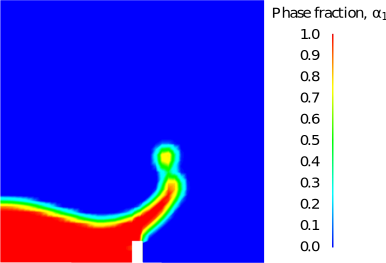
\includegraphics{fig-2-22-a}\par
 (a) $t = 0.25\unit{s}$のとき\par
 \medskip
 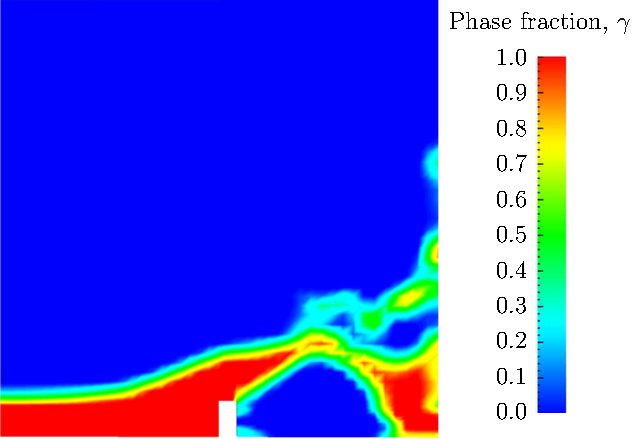
\includegraphics{fig-2-22-b}\par
 (b) $t = 0.50\unit{s}$のとき
 \caption{$\alpha_{1}$相のスナップショット}
 \label{fig:2.22}
\end{figure}


\subsection{並列計算}
\label{ssec:2.3.10}
前述の例の結果はかなり目の粗い格子を使って得られました.
ここでは格子の解像度を増やして再計算します.
新しいケースは,一般的に一つのプロセッサでは
計算するのに数時間を要するので,
複数のプロセッサにアクセスしているのであれば,
OpenFOAMの並列計算機能を試してみてもよいでしょう.

まず初めに,\OFcase{damBreak}ケースのコピーをしてください.
\begin{OFverbatim}[terminal]
cd $FOAM_RUN/tutorials/interFoam
mkdir damBreakFine
cp -r damBreak/0 damBreakFine
cp -r damBreak/system damBreakFine
cp -r damBreak/constant damBreakFine
\end{OFverbatim}%$

新しいケースは\OFcase{damBreakFine}と名づけてください.
新しいケースディレクトリを開いて
\OFdictionary{blockMeshDict}ファイル内の
\OFkeyword{blocks}の記述を以下のように変更してください.
\begin{OFverbatim}[file]
blocks
(
    hex (0 1 5 4 12 13 17 16) (46 10 1) simpleGrading (1 1 1)
    hex (2 3 7 6 14 15 19 18) (40 10 1) simpleGrading (1 1 1)
    hex (4 5 9 8 16 17 21 20) (46 76 1) simpleGrading (1 2 1)
    hex (5 6 10 9 17 18 22 21) (4 76 1) simpleGrading (1 2 1)
    hex (6 7 11 10 18 19 23 22) (40 76 1) simpleGrading (1 2 1)
);
\end{OFverbatim}
上記で,入力は\OFdictionary{blockMeshDict}ファイルで表示されているように,
つまりは,格子の密度を変更しなければなりません.
例えば\texttt{46 10 1}という入力や\texttt{1 2 1}という格子幅の勾配の入力のようにです.
正しく入力できたら,メッシュを生成します.

ここで格子が\OFcase{damBreak}の例から変更されると,
時刻\OFpath{0}のディレクトリ内の\OFpath{alpha1}という相の場を
再初期化しなければなりません.
というのも\OFkeyword{alpha1}は新しい格子とは合致しない
いくつかの要素を含んでいるからです.
ここで,\OFkeyword{U}や\OFkeyword{p\_rgh}という場は
変更する必要がないことに注意しましょう.
それらは\OFkeyword{uniform}として明記されており
フィールド内の要素の数と独立だからです.
フィールドの初期化はシャープな界面を持つように行いたいものです.
つまり,その要素が$\alpha_{1} = 1$または$\alpha_{1} = 0$となるようにです.
\OFtool{mapFields}によりフィールドを更新すると,
界面に補間された$0 < \alpha_{1} < 1$となる値が生成される可能性があるので,
\OFtool{setFields}ユーティリティを再実行したほうがよいでしょう.
その前に初期条件の一様な$\alpha_{1}$のバックアップファイル
\OFpath{0/alpha1.org}を\OFpath{0/alpha1}にコピーします.
\begin{OFverbatim}[terminal]
cd $FOAM_RUN/tutorials/interFoam/laminar/damBreakFine
cp -r 0/alpha1.org 0/alpha1
setFields
\end{OFverbatim}%$

OpenFOAMで用いられる並列計算の手法はいわゆる領域分割であり,
幾何形状やそれに関連する場が領域ごとに分解されて,
解析のため個々のプロセッサに割り当てられます.
そのため,並列計算を実行するために必要な最初の段階は,
\OFtool{decomposePar}を用いて領域を分解することです.
\OFtool{decomposePar}の設定は\OFpath{system}ディレクトリにある,
\OFdictionary{decomposeParDict}というファイルです.
他のユーティリティ同様,初期状態のファイルが
ユーティリティのソースコードの
ディレクトリ (\OFpath{\$FOAM\_UTILITIES/parallelProcessing/\allowbreak decomposePar}) にあります.

最初の入力の\OFkeyword{numberOfSubdomains}において
何個のサブ領域に分割するかを指定します.
通常はこのケースに利用できるプロセッサの数と対応します.

このチュートリアルでは,分解の手法は\OFkeyword{simple}で,
対応する\OFkeyword{simpleCoeffs}は以下の基準のように編集しましょう.
領域は,$x$,$y$,$z$方向で部分かサブ領域に分けられ,
各方向へのサブ領域の数はベクトル$\bm{n}$として与えられます.
この幾何形状は2次元なので,3番目の方向$z$に分割されることはなく,
それゆえ必ず$n_{z}$は$1$になります.
$n_{x}$と$n_{y}$は$x$,$y$方向の領域の分割数$\bm{n}$を構成し,
$n_{x}$と$n_{y}$の積で表されるサブ領域の数が\OFkeyword{numberOfSubdomain}に指定したものと
等しくなる必要があります.
隣接するサブ領域間のセル面の数を最小にしたほうがよいので,
正方形の幾何形状では,$x$,$y$方向を均等に分割するのが良いでしょう.
\OFkeyword{delta}キーワードは\OFkeyword{0.001}に設定しましょう.

例として,四つのプロセッサで計算を実行するとします.
\OFkeyword{numberOfSubdomain}を4に,$\bm{n} = (2, 2, 1)$に設定します.
\OFdictionary{decomposeParDict}を閉じて,\OFtool{decomposePar}を実行します.
\OFtool{decomposePar}のスクリーンメッセージが確認でき,
分解はプロセッサ間で均等に分配されたと表示されます.

\autoref{sec:3.4}に
並列計算の方法についての詳細があるので参照してください.
このチュートリアルでは並列計算の一例を示しているにすぎません.
openMPIを用いて標準のメッセージパッシングインターフェース (MPI) を
実装しています.
ここでは,テストとしてローカルホストのみの単独ノードで実行します.
\begin{OFverbatim}[terminal]
mpirun -np 4 interFoam -parallel > log &
\end{OFverbatim}
\autoref{ssec:3.4.2}に後述しますが,
ケースが実行されるマシンのホストネームを列記したファイルを作っておけば
ネットワーク上のより多くのノードを使って計算することも可能です.
ケースはバックグラウンドで実行し,
進行状況を\OFpath{log}ファイルで監視するのがよいでしょう.


\begin{figure}[ht]
 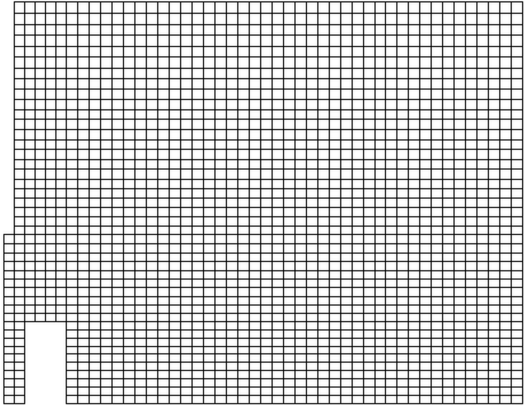
\includegraphics{fig-2-23}
 \caption{並列プロセスケースでのプロセッサ2のメッシュ}
 \label{fig:2.23}
\end{figure}


\begin{figure}[ht]
 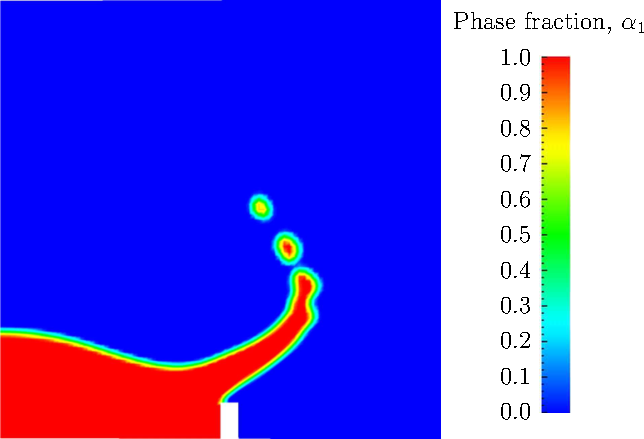
\includegraphics{fig-2-24-a}\par
 (a) $t = 0.25\unit{s}$のとき\par
 \medskip
 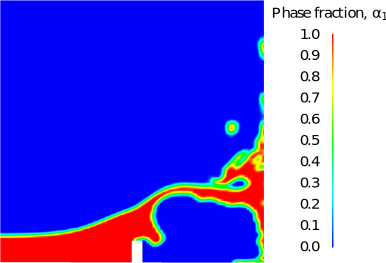
\includegraphics{fig-2-24-b}\par
 (b) $t = 0.50\unit{s}$のとき
 \caption{正確なメッシュの$\alpha_{1}$相のスナップショット}
 \label{fig:2.24}
\end{figure}


\subsection{並列計算ケースの後処理}
\label{sssec:2.3.11}
一度ケースの実行が完了したら,
分解されたフィールドとメッシュは\OFtool{reconstructPar}を実行して
後処理のために再統合します.
コマンドラインから容易に実行できます.
細かい格子による結果は\autoref{fig:2.24}に表されます.
インタフェースでの結果は粗い格子のものと比較して
著しく改良されたことがみてとれます.

また,単に個々のプロセッサの領域を一つのケースと扱うことで,
分解された領域の部分を個々に後処理することもできます.

例えば,\OFtool{paraFoam}を以下のように起動します.
\begin{OFverbatim}[terminal]
paraFoam -case processor1
\end{OFverbatim}
すると\OFkeyword{processor1}が\OFthirdparty{ParaView}のケースモジュールとして表れます.
\autoref{fig:2.23}に,\OFkeyword{simple}方式による領域分割を行った際の
\OFkeyword{processor1}のメッシュを示します.
